%%%%%%%%%%%%%%%%%%%%%%%%%%%%%%%%%%%%%%%%%%%%%%%%%%%%%%%%%%%%%%%%%%%%%%%%
%% Customizações do abnTeX2 (http://abnTeX2.googlecode.com)           %%
%% para a Universidade Estadual do Ceara - UECE                       %%
%%                                                                    %%
%% This work may be distributed and/or modified under the             %% 
%% conditions of the LaTeX Project Public License, either version 1.3 %%
%% of this license or (at your option) any later version.             %%
%% The latest version of this license is in                           %%
%%   http://www.latex-project.org/lppl.txt                            %%
%% and version 1.3 or later is part of all distributions of LaTeX     %%
%% version 2005/12/01 or later.                                       %%
%%                                                                    %%
%% This work has the LPPL maintenance status `maintained'.            %%
%%                                                                    %%
%% The Current Maintainer of this work is Thiago Nascimento           %%
%%                                                                    %%
%% Project available on: https://github.com/thiagodnf/uecetex2        %%
%%                                                                    %%
%% Further information about abnTeX2                                  %%
%% are available on http://abntex2.googlecode.com/                    %%
%%                                                                    %%
%%%%%%%%%%%%%%%%%%%%%%%%%%%%%%%%%%%%%%%%%%%%%%%%%%%%%%%%%%%%%%%%%%%%%%%%

% Preâmbulo do documento

%%%%%%%%%%%%%%%%%%%%%%%%%%%%%%%%%%%%%%%%%%%%%%%%%%%%%%%%%%%%%%%%%%%%%%%%
%% Customizações do abnTeX2 (http://abnTeX2.googlecode.com)           %%
%% para a Universidade Estadual do Ceara - UECE                       %%
%%                                                                    %%
%% This work may be distributed and/or modified under the             %% 
%% conditions of the LaTeX Project Public License, either version 1.3 %%
%% of this license or (at your option) any later version.             %%
%% The latest version of this license is in                           %%
%%   http://www.latex-project.org/lppl.txt                            %%
%% and version 1.3 or later is part of all distributions of LaTeX     %%
%% version 2005/12/01 or later.                                       %%
%%                                                                    %%
%% This work has the LPPL maintenance status `maintained'.            %%
%%                                                                    %%
%% The Current Maintainer of this work is Thiago Nascimento           %%
%%                                                                    %%
%% Project available on: https://github.com/thiagodnf/uecetex2        %%
%%                                                                    %%
%% Further information about abnTeX2                                  %%
%% are available on http://abntex2.googlecode.com/                    %%
%%                                                                    %%
%%%%%%%%%%%%%%%%%%%%%%%%%%%%%%%%%%%%%%%%%%%%%%%%%%%%%%%%%%%%%%%%%%%%%%%%

\documentclass[        
    a4paper,          % Tamanho da folha A4
    12pt,             % Tamanho da fonte 12pt
    chapter=TITLE,    % Todos os capitulos devem ter caixa alta
    section=TITLE,    % Todas as secoes devem ter caixa alta
    oneside,          % Usada para impressao em apenas uma face do papel
    english,          % Hifenizacoes em ingles
    spanish,          % Hifenizacoes em espanhol
    brazil            % Ultimo idioma eh o idioma padrao do documento
]{abntex2}

% Importações de pacotes
\usepackage[utf8]{inputenc}                         % Acentuação direta
\usepackage[T1]{fontenc}                            % Codificação da fonte em 8 bits
\usepackage{graphicx}                               % Inserir figuras
\usepackage{amsfonts, amssymb, amsmath}             % Fonte e símbolos matemáticos
\usepackage{booktabs}                               % Comandos para tabelas
\usepackage{verbatim}                               % Texto é interpretado como escrito no documento
\usepackage{multirow, array}                        % Múltiplas linhas e colunas em tabelas
\usepackage{indentfirst}                            % Endenta o primeiro parágrafo de cada seção.
\usepackage{listings}                               % Utilizar codigo fonte no documento
\usepackage{xcolor}
\usepackage{microtype}                              % Para melhorias de justificação?
\usepackage[portuguese,ruled,lined]{algorithm2e}    % Escrever algoritmos
\usepackage{algorithmic}                            % Criar Algoritmos  
\usepackage{float}									% Utilizado para criação de floats
\usepackage{newfloat}                                
\usepackage{amsgen}
\usepackage{lipsum}                                 % Usar a simulação de texto Lorem Ipsum
%\usepackage{titlesec}                              % Permite alterar os títulos do documento
\usepackage{tocloft}                                % Permite alterar a formatação do Sumário
\usepackage{etoolbox}                               % Usado para alterar a fonte da Section no Sumário
\usepackage[nogroupskip,nonumberlist,acronym]{glossaries}                % Permite fazer o glossario
\usepackage{caption,setspace}                                % Altera o comportamento da tag caption
\usepackage[alf, abnt-emphasize=bf, bibjustif, recuo=0cm, abnt-etal-cite=3, abnt-etal-list=0,abnt-etal-text=it]{abntex2cite}  % Citações padrão ABNT
%\usepackage[bottom]{footmisc}                      % Mantém as notas de rodapé sempre na mesma posição
%\usepackage{times}                                 % Usa a fonte Times
\usepackage{mathptmx}                               % Usa a fonte Times New Roman										
%\usepackage{lmodern}                               % Usa a fonte Latin Modern
%\usepackage{subfig}                                % Posicionamento de figuras
%\usepackage{scalefnt}                              % Permite redimensionar tamanho da fonte
%\usepackage{color, colortbl}                       % Comandos de cores
%\usepackage{lscape}                                % Permite páginas em modo "paisagem"
%\usepackage{ae, aecompl}                           % Fontes de alta qualidade
%\usepackage{picinpar}                              % Dispor imagens em parágrafos
%\usepackage{latexsym}                              % Símbolos matemáticos
%\usepackage{upgreek}                               % Fonte letras gregas
\usepackage{appendix}                               % Gerar o apendice no final do documento
\usepackage{paracol}                                % Criar paragrafos sem identacao
\usepackage{pdfpages}                               % Incluir pdf no documento
\usepackage{amsmath}                                % Usar equacoes matematicas
\usepackage{hyperref}								% formatação de hiperlinks
\usepackage{setspace}								% Configuração de espaçamentos
%================================================================================================================
\usepackage{lib/uecetex2}		                    % Biblioteca com as normas da UECE para trabalhos academicos
%================================================================================================================

% Organiza e gera a lista de abreviaturas, simbolos e glossario
\makeglossaries

% Gera o Indice do documento
\makeindex


%%%%%%%%%%%%%%%%%%%%%%%%%%%%%%%%%%%%%%%%%%%%%%%%%%%%%%%%%%
%%    Configuracoes do ueceTeX2 abaptado para o IFCE    %%
%%%%%%%%%%%%%%%%%%%%%%%%%%%%%%%%%%%%%%%%%%%%%%%%%%%%%%%%%%

% Opcoes disponiveis

\trabalhoacademico{tccgraduacao}
%\trabalhoacademico{tccespecializacao}
%\trabalhoacademico{dissertacao}
%\trabalhoacademico{tese}

% Define se o trabalho eh uma qualificacao
% Coloque 'nao' para versao final do trabalho

\ehqualificacao{nao}

% Remove as bordas vermelhas e verdes do PDF gerado
% Coloque 'sim' pare remover

\removerbordasdohyperlink{sim} 

% Adiciona a cor Azul a todos os hyperlinks

\cordohyperlink{nao}

%%%%%%%%%%%%%%%%%%%%%%%%%%%%%%%%%%%%%%%%%%%%%%%%%%%%%
%%          Informação sobre a IES                 %%
%%%%%%%%%%%%%%%%%%%%%%%%%%%%%%%%%%%%%%%%%%%%%%%%%%%%%

\ies{Instituto Federal de Educação, Ciência e Tecnologia do Ceará}
\iessigla{IFCE}
\campus{Tauá}
\centro{}
%%%%%%%%%%%%%%%%%%%%%%%%%%%%%%%%%%%%%%%%%%%%%%%%%%%%%
%%        Informação para TCC de Graduacao         %%
%%%%%%%%%%%%%%%%%%%%%%%%%%%%%%%%%%%%%%%%%%%%%%%%%%%%%

\graduacaoem{Tecnologia em Telemática}
\habilitacao{bacharel} % Pode colocar tambem 'licenciada'

%%%%%%%%%%%%%%%%%%%%%%%%%%%%%%%%%%%%%%%%%%%%%%%%%%%%%
%%     Informação para TCC de Especializacao       %%
%%%%%%%%%%%%%%%%%%%%%%%%%%%%%%%%%%%%%%%%%%%%%%%%%%%%%

\especializacaoem{Alfabetização de Crianças}

%%%%%%%%%%%%%%%%%%%%%%%%%%%%%%%%%%%%%%%%%%%%%%%%%%%%%
%%         Informação para Dissertacao             %%
%%%%%%%%%%%%%%%%%%%%%%%%%%%%%%%%%%%%%%%%%%%%%%%%%%%%%

\programamestrado{Programa de Pós-Graduação em Ciência da Computação}
\nomedomestrado{Mestrado Acadêmico em Ciência da Computação}
\mestreem{Ciência da Computação}
\areadeconcentracaomestrado{Ciência da Computação}

%%%%%%%%%%%%%%%%%%%%%%%%%%%%%%%%%%%%%%%%%%%%%%%%%%%%%
%%               Informação para Tese              %%
%%%%%%%%%%%%%%%%%%%%%%%%%%%%%%%%%%%%%%%%%%%%%%%%%%%%%

\programadoutorado{Programa de Pós-Graduação em Saúde Coletiva}
\nomedodoutorado{Doutorado em Saúde Coletiva}
\doutorem{Saúde Coletiva}
\areadeconcentracaodoutorado{Saúde Coletiva}

%%%%%%%%%%%%%%%%%%%%%%%%%%%%%%%%%%%%%%%%%%%%%%
%%  Informação relacionadas ao trabalho     %%
%%%%%%%%%%%%%%%%%%%%%%%%%%%%%%%%%%%%%%%%%%%%%%

\autor{Leonardo Feitosa Nogueira}
\titulo{Título do Trabalho}
\data{2019}
\local{Tauá -- Ceará}

% Exemplo: \dataaprovacao{01 de Janeiro de 2012}
\dataaprovacao{}

%%%%%%%%%%%%%%%%%%%%%%%%%%%%%%%%%%%%%%%%%%%%%%%
%%     Informação sobre o Orientador(a)      %%
%%%%%%%%%%%%%%%%%%%%%%%%%%%%%%%%%%%%%%%%%%%%%%%

\orientador{Prof. Dr. Francisco Rafael Vasconcelos Guimarães}
\orientadories{Instituto Federal de Educação, Ciência e Tecnologia do Ceará -- IFCE}
\orientadorcentro{}
\orientadorfeminino{nao} % Coloque 'sim' se for do sexo feminino

%%%%%%%%%%%%%%%%%%%%%%%%%%%%%%%%%%%%%%%%%%%%%%%
%%      Informação sobre o Coorientador(a)   %%
%%%%%%%%%%%%%%%%%%%%%%%%%%%%%%%%%%%%%%%%%%%%%%%

% Deixe o nome do coorientador em branco para remover do documento

\coorientador{Prof. Kilbert Amorim Maciel}
\coorientadories{Instituto Federal de Educação, Ciência e Tecnologia do Ceará -- IFCE}
\coorientadorcentro{}
\coorientadorfeminino{nao} % Coloque 'sim' se for do sexo feminino

%%%%%%%%%%%%%%%%%%%%%%%%%%%%%%%%%%%%%%%%%%%%%%%
%%      Informação sobre a banca             %%
%%%%%%%%%%%%%%%%%%%%%%%%%%%%%%%%%%%%%%%%%%%%%%%

% Atenção! Deixe o nome do membro da banca em branco para remover da folha de aprovacao

% Exemplo de uso:
% \membrodabancadois{Prof. Dr. Fulano de Tal}
% \membrodabancadoisies{Universidade Estadual do Ceará - UECE}

\membrodabancadois{Membro da Banca Dois}
\membrodabancadoiscentro{Faculdade de Filosofia Dom Aureliano Matos – FAFIDAM}
\membrodabancadoisies{Universidade do Membro da Banca Dois - SIGLA}
\membrodabancatres{Membro da Banca Três}
\membrodabancatrescentro{Centro de Ciências e Tecnologia - CCT}
\membrodabancatresies{Universidade do Membro da Banca Três - SIGLA}
\membrodabancaquatro{Membro da Banca Quatro}
\membrodabancaquatrocentro{Centro de Ciências e Tecnologia - CCT}
\membrodabancaquatroies{Universidade do Membro da Banca Quatro - SIGLA}
\membrodabancacinco{Membro da Banca Cinco}
\membrodabancacincocentro{Teste}
\membrodabancacincoies{Universidade do Membro da Banca Cinco - SIGLA}
\membrodabancaseis{Membro da Banca Seis}
\membrodabancaseiscentro{}
\membrodabancaseisies{Universidade do Membro da Banca Seis - SIGLA}

\begin{document}	

	% Se o seu trabalho é em ingles, descomente a linha a seguir
	%\selectlanguage{english}

	% Elementos pré-textuais
	\imprimircapa
	\imprimirfolhaderosto{}
	\imprimirfichacatalografica{elementos-pre-textuais/ficha-catalografica}
	\imprimirerrata{elementos-pre-textuais/errata}
	\imprimirfolhadeaprovacao
	\imprimirdedicatoria{elementos-pre-textuais/dedicatoria}
	\imprimiragradecimentos{elementos-pre-textuais/agradecimentos}
	\imprimirepigrafe{elementos-pre-textuais/epigrafe}
	\imprimirresumo{elementos-pre-textuais/resumo}
	\imprimirabstract{elementos-pre-textuais/abstract}
	\imprimirlistadeilustracoes
	\imprimirlistadetabelas
	%\imprimirlistadequadros
	%\imprimirlistadealgoritmos
	%\imprimirlistadecodigosfonte
	\imprimirlistadeabreviaturasesiglas{elementos-pre-textuais/lista-de-abreviaturas-e-siglas}
	\imprimirlistadesimbolos{elementos-pre-textuais/lista-de-simbolos}   
	\imprimirsumario
	
	% Elementos textuais
	\textual
	% Arquivos de Exemplo
	\chapter{Introdução}
\label{cap:introducao}

Em 1971, o sistema Aloha\footnote{Originalmente, o sistema Aloha, desenvolvido por Norman Abramson em 1970, na Universidade do Havaí, funcionava como um protocolo para sistemas de comunicação via radiofrequência para o acesso remoto entre computadores enviando pacotes num sistema de radiocomunicação \cite{abramson1970acm, haykin2009}.} estabeleceu e operou uma rede de dados terrestres (AlohaNet) no estado americano do Havaí. Em 1973, ao sofrer uma adaptação, o sistema Aloha usou um transponder acoplada em um satélite experimental da Agência Espacial Americana (NASA, do inglês, \textit{National Aeronautics and Space Administration}) (ATS-1) para demonstrar uma rede internacional de dados via satélite conectando a NASA, na Califórnia, e cinco universidades nos Estados Unidos, Japão e Austrália, fornecendo a primeira demonstração pública de uma rede de dados por pacotes sem fio \cite{abramson1970acm, SchwartzAbramson2009ieee}. Também em 1973, o rede AlohaNet foi vinculada à ARPANet\footnote{A primeira rede de computadores por comutação de pacotes e uma ancestral direta da Internet pública de hoje \cite{kurose2013}.} (do inglês, \textit{Advanced Research Projects Agency Network}) \cite{abramson1970acm, SchwartzAbramson2009ieee}.

Mesmo com limitações como largura de banda e tecnologia de transmissão, foi graças ao pioneirismo do sistema Aloha, que as redes de comutação sem fio, conhecidas como \textit{wireless} ou ainda WLANs (do inglês, \textit{Wireless Local Area Network}) surgiram como redes complementares às redes cabeadas tradicionais. Essa tecnologia de comunicação se desenvolveu devido a necessidade de implementação de um método alternativo de conexão que não privasse a movimentação do usuário a uma posição fixa durante uma transmissão/recepção de dados na rede. O tempo passou e a tecnologia evoluiu, deixou de ser restrito ao meio acadêmico e militar e se tornou acessível a empresas e ao usuário doméstico. Nos dias de hoje podemos pensar em redes \textit{wireless} como uma alternativa bastante interessante em relação às redes cabeadas. Suas aplicações são muitas e variadas e o fato de ter a mobilidade como principal característica, tem facilitado a sua aceitação, principalmente nas empresas (FARIAS, 2005).

Com o advento de \textit{notebooks}, \textit{tablets}, \textit{smartphones} e a promessa de acesso desimpedido à Internet global de qualquer lugar por meio das comunicações sem fio, a qualquer hora, assistimos a uma explosão semelhante da utilização de dispositivos sem fio para acesso à Internet em comparação ao dos telefones móveis, não só através da rede de telefonia móvel, agora plenamente possível, mas também por meio das redes Wi-Fi. O uso deste tipo de rede está se tornando cada vez mais comum, não só nos ambientes domésticos e corporativos, mas também em locais públicos (bares, lanchonetes, shoppings, aeroportos, etc) e em instituições acadêmicas. Independentemente do crescimento futuro de equipamentos sem fio para Internet, já ficou claro que as redes sem fio e os serviços móveis relacionados que elas possibilitam vieram para ficar (KUROSE; ROSS, 2013; GAST, 2002).

No período em que as redes locais cabeadas (LAN -- \textit{Local Area Network}, do inglês)  dominavam a infraestrutura de rede de computadores, somente era possível conectar computadores à Internet e entre si por meio de cabos padrão Ethernet. Este tipo de conexão é bastante popular, mas conta com algumas limitações, por exemplo: só se pode movimentar o computador até o limite de alcance do cabo; ambientes com um grande número computadores podem exigir adaptações na estrutura do prédio para a passagem dos fios; em uma residência, pode ser necessário realizar perfurações na parede para que os cabos alcancem outros cômodos; a manipulação constante ou incorreta pode fazer com que o conector do cabo de rede se danifique. Com exceção da mobilidade, o restante das alegações implica em investimento financeiro direto por parte das empresas e também para o usuário doméstico. Felizmente, as redes sem fio Wi-Fi surgiram para eliminar estas limitações. Como consequência, alcançaram rapidamente uma disseminação generalizada tanto no espaço comercial quanto no residencial (ALECRIM, 2008).

%\lipsum[5]
%\lipsum[6]
%\lipsum[7]

\newpage
\section{Motivação}
\label{sec:motivacao}

%\lipsum[3]
%\lipsum[4]

\section{Objetivos}
\label{sec:objetivos}

Interdum et malesuada fames ac ante ipsum primis in faucibus. Lorem ipsum dolor sit amet, consectetur adipiscing elit. Ut ex tellus, sodales in euismod at, ultricies quis leo \cite{alecrim2008site}.

\subsection{Objetivo Geral}
\label{sec:objetivo-geral}

Integer imperdiet ac magna eu pulvinar. Aliquam erat volutpat. Etiam molestie, nulla a egestas aliquet, velit augue congue metus, et ultricies metus massa vel nibh. Vivamus viverra commodo finibus. Nam elementum convallis accumsan. Quisque tincidunt purus nisl, tincidunt ultricies odio ultrices eu.

\subsection{Objetivos Específicos}
\label{sec:objetivos-especificos}

Lorem ipsum dolor sit amet, consectetur adipiscing elit. Duis scelerisque, velit at facilisis hendrerit, dui eros lacinia metus, non maximus mi tortor ut lectus. Donec hendrerit leo ut consectetur tincidunt. 

	\begin{alineas}
		\item Lorem ipsum dolor sit amet, consectetur adipiscing elit. Nunc dictum sed tortor nec viverra.
		\item Praesent vitae nulla varius, pulvinar quam at, dapibus nisi. Aenean in commodo tellus. Mauris molestie est sed justo malesuada, quis feugiat tellus venenatis.
		\item Praesent quis erat eleifend, lacinia turpis in, tristique tellus. Nunc dictum sed tortor nec viverra.
		\item Mauris facilisis odio eu ornare tempor. Nunc dictum sed tortor nec viverra.
		\item Curabitur convallis odio at eros consequat pretium.
	\end{alineas}
	\chapter{Fundamentação Teórica}
\label{cap:fundamentacao-teorica}

Integer non lacinia magna. Aenean tempor lorem tellus, non sodales nisl commodo ut. Proin mattis placerat risus sit amet laoreet. Praesent sapien arcu, maximus ac fringilla efficitur, vulputate faucibus sem. Donec aliquet velit eros, sit amet elementum dolor pharetra eget. Integer eget mattis libero

\section{Fundamentação Teórica A}
\label{sec:fundamentacao-teorica-a}

\lipsum[10]

	\begin{figure}[h!]
		\centering
		\Caption{\label{fig:exemplo-1} Lorem ipsum dolor sit amet, consectetur adipiscing elit. Suspendisse commodo lectus et augue elementum varius.}	
		\UECEfig{}{
			\fbox{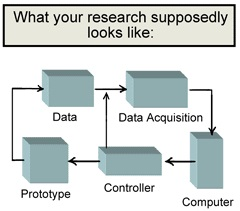
\includegraphics[width=8cm]{figuras/figura-1}}
		}{
			\Fonte{Elaborado pelo autor}
		}	
	\end{figure}
	
\lipsum[11]


\section{Fundamentação Teórica B}
\label{sec:fundamentacao-teorica-b}

Integer non lacinia magna. Aenean tempor lorem tellus, non sodales nisl commodo ut. Proin mattis placerat risus sit amet laoreet. Praesent sapien arcu, maximus ac fringilla efficitur, vulputate faucibus sem. Donec aliquet velit eros, sit amet elementum dolor pharetra eget. Integer eget mattis libero. Praesent ex velit, pulvinar at massa vel, fermentum dictum mauris. Ut feugiat accumsan augue, et ultrices ipsum euismod vitae

	\begin{figure}[h!]
		\centering
		\Caption{\label{fig:exemplo-2} Maecenas luctus augue odio, sed tincidunt nunc posuere nec}	
		\UECEfig{}{
			\fbox{
\includegraphics[width=8cm]{figuras/figura-2}}
		}{
			\Fonte{Elaborado pelo autor}			
		}	
	\end{figure}

Nunc ac pretium dui. Mauris aliquam dapibus nulla ac mattis. Aenean non tortor volutpat, varius lectus vitae, accumsan nibh. Cras pretium vestibulum enim, id ullamcorper tortor ultrices non. Integer sodales viverra faucibus. Curabitur at dui lacinia, rhoncus lacus at, blandit metus. Integer scelerisque non enim quis ornare.

\lipsum[13]

	\begin{table}[h!]	
		\centering
		\Caption{\label{tab:exemplo-1} Duis faucibus, enim quis tincidunt pellentesque, nisl leo varius nulla, vitae tempus dui mauris ac ante purus lorem}		
		\UECEtab{}{
			\begin{tabular}{cll}
				\toprule
				Ranking & Exon Coverage & Splice Site Support \\
				\midrule \midrule
				E1 & Complete coverage by a single transcript & Both splice sites\\
				E2 & Complete coverage by more than a single transcript & Both splice sites\\
				E3 & Partial coverage & Both splice sites\\
				E4 & Partial coverage & One splice site\\
				E5 & Complete or partial coverage & No splice sites\\
				E6 & No coverage & No splice sites\\
				\bottomrule
			\end{tabular}
		}{
		\Fonte{Elaborado pelo autor}
	}
	\end{table}

Duis faucibus, enim quis tincidunt pellentesque, nisl leo varius nulla, vitae tempus dui mauris ac ante. Quisque purus lorem, pharetra sit amet lobortis eu, vehicula vitae purus. Ut varius, erat nec vehicula elementum, risus est tempus justo, nec vulputate augue leo egestas metus.

	\begin{figure}[h!]
		\centering
		\Caption{\label{fig:exemplo-3} Ut posuere, ex quis sagittis auctor, magna massa euismod felis}	
		\UECEfig{}{
			\fbox{
\includegraphics[width=8cm]{figuras/figura-2}}
		}{
		\Fonte{Elaborado pelo autor}			
	}	
	\end{figure}

\lipsum[14]

	\begin{table}[h!]	
		\centering
		\Caption{\label{tab:exemplo-2} Etiam molestie, nulla a egestas aliquet, velit augue congue metus}		
		\UECEtab{}{
			\begin{tabular}{ccll}
				\toprule
				Quisque & pharetra & tempus & vulputate \\
				\midrule \midrule
				E1 & Complete coverage by a single transcript & Both splice sites\\
				E2 & Complete coverage by more than a single transcript & Both splice sites\\
				E3 & Partial coverage & Both splice sites & Both \\
				E4 & Partial coverage & One splice site & Both \\
				E5 & Complete or partial coverage & No splice sites & Both\\
				E6 & No coverage & No splice sites\\
				\bottomrule
			\end{tabular}
		}{
		\Fonte{Elaborado pelo autor}
	}
	\end{table}
	
Duis faucibus, enim quis tincidunt pellentesque, nisl leo varius nulla, vitae tempus dui mauris ac ante. Quisque purus lorem, pharetra sit amet lobortis eu, vehicula vitae purus.
\acrlong{DATASUS},\acrlong{DNV},\acrlong{DO},\acrlong{ESF},\acrlong{IBGE},\acrlong{MFC},\acrlong{MI},\acrlong{MS},\acrlong{NV},\acrlong{ODM},\acrlong{OI},\acrlong{OMS},\acrlong{ONU},\acrlong{PNI},\acrlong{PSF},\acrlong{RIPSA},\acrlong{RN},\acrlong{SIM},\acrlong{SINASC},\acrlong{SUS},\acrlong{TMI},\acrlong{TMMFC}

\begin{alineascomponto}
	\item Integer non lacinia magna. Aenean tempor lorem tellus, non sodales nisl commodo ut
	\item Proin mattis placerat risus sit amet laoreet. Praesent sapien arcu, maximus ac fringilla efficitur, vulputate faucibus sem. Donec aliquet velit eros, sit amet elementum dolor pharetra eget
	\item Integer eget mattis libero. Praesent ex velit, pulvinar at massa vel, fermentum dictum mauris. Ut feugiat accumsan augue, et ultrices ipsum euismod vitae
	\begin{subalineascomponto}
		\item Integer non lacinia magna. Aenean tempor lorem tellus, non sodales nisl commodo ut
		\item Proin mattis placerat risus sit amet laoreet.
	\end{subalineascomponto}
\end{alineascomponto}
	\chapter{Trabalhos Relacionados}
\label{cap:trabalhos-relacionados}

Integer non lacinia magna. Aenean tempor lorem tellus, non sodales nisl commodo ut. Proin mattis placerat risus sit amet laoreet. Praesent sapien arcu, maximus ac fringilla efficitur, vulputate faucibus sem. Donec aliquet velit eros, sit amet elementum dolor pharetra eget. Integer eget mattis libero

\section{Trabalho Relacionado A}
\label{sec:trabalho-relacionado-a}

\lipsum[10]

	\begin{figure}[h!]
		\centering
		\Caption{\label{fig:exemplo-1} Lorem ipsum dolor sit amet, consectetur adipiscing elit. Suspendisse commodo lectus et augue elementum varius.}	
		\UECEfig{}{
			\fbox{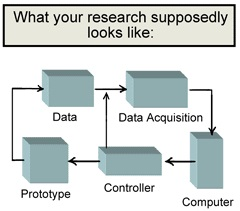
\includegraphics[width=8cm]{figuras/figura-1}}
		}{
			\Fonte{Elaborado pelo autor}
		}	
	\end{figure}
	
\lipsum[11]

\section{Trabalho Relacionado B}
\label{sec:trabalho-relacionado-b}

Integer non lacinia magna. Aenean tempor lorem tellus, non sodales nisl commodo ut. Proin mattis placerat risus sit amet laoreet. Praesent sapien arcu, maximus ac fringilla efficitur, vulputate faucibus sem. Donec aliquet velit eros, sit amet elementum dolor pharetra eget. Integer eget mattis libero. Praesent ex velit, pulvinar at massa vel, fermentum dictum mauris. Ut feugiat accumsan augue, et ultrices ipsum euismod vitae

	\begin{figure}[h!]
		\centering
		\Caption{\label{fig:exemplo-2} Maecenas luctus augue odio, sed tincidunt nunc posuere nec}	
		\UECEfig{}{
			\fbox{
\includegraphics[width=8cm]{figuras/figura-2}}
		}{
			\Fonte{Elaborado pelo autor}			
		}	
	\end{figure}

Nunc ac pretium dui. Mauris aliquam dapibus nulla ac mattis. Aenean non tortor volutpat, varius lectus vitae, accumsan nibh. Cras pretium vestibulum enim, id ullamcorper tortor ultrices non. Integer sodales viverra faucibus. Curabitur at dui lacinia, rhoncus lacus at, blandit metus. Integer scelerisque non enim quis ornare.

	\begin{quadro}[h!]	
		\centering
		\Caption{\label{qua:exemplo-1} Praesent ex velit, pulvinar at massa vel, fermentum dictum mauris. Ut feugiat accumsan augue}		
		\UECEqua{}{
			\begin{tabular}{|c|c|l|l|}
				\hline
				Quisque & pharetra & tempus & vulputate \\
				\hline
				E1 & Complete coverage by a single transcript & Both  & Complete\\
				\hline
				E2 & Complete coverage by more than & Both splice sites & Complete\\
				\hline
				E3 & Partial coverage & Both splice sites & Both \\				
				\hline
			\end{tabular}
		}{
			\Fonte{Elaborado pelo autor}
		}
	\end{quadro}
	
\lipsum[20]

	
	\begin{quadro}[h!]	
		\centering
		\Caption{\label{qua:exemplo-2} Duis faucibus, enim quis tincidunt pellentesque}		
		\UECEqua{}{
			\begin{tabular}{|c|c|}
				\hline
				Quisque & pharetra \\
				\hline
				E1 & Complete coverage by a single transcript \\
				\hline
				E2 & Complete coverage by more than \\
				\hline
				E3 & Partial coverage \\
				\hline
				E4 & Partial coverage \\
				\hline
				E5 & Partial coverage \\
				\hline
				E6 & Partial coverage \\
				\hline
				E7 & Partial coverage \\
				\hline
			\end{tabular}
		}{
			\Fonte{Elaborado pelo autor}
		}
	\end{quadro}

\lipsum[21]

Integer non lacinia magna. Aenean tempor lorem tellus, non sodales nisl commodo ut. Proin mattis placerat risus sit amet laoreet. Praesent sapien arcu, maximus ac fringilla efficitur, vulputate faucibus sem. Donec aliquet velit eros, sit amet elementum dolor pharetra eget. Integer eget mattis libero.
\Gls{ambiguidade}
\Gls{braile}
\Gls{coerencia}
\Gls{dialetos}
\Gls{elipse}
\Gls{locucao-adjetiva}
\Gls{modificadores}
\Gls{paronimos}
\Gls{sintese}
\Gls{borboleta}
	\chapter{Metodologia}
\label{chap:metodologia}

\lipsum[2]
\lipsum[12]

O autor \cite{lamport1986latex} e \cite{Maia2011} \lipsum[2] 

\begin{table}[h!]
	\Caption{\label{tabela-ibge} Um Exemplo de tabela alinhada que pode ser longa ou curta, conforme padrão IBGE. conforme padrão IBGE. conforme padrão IBGE. conforme padrão IBGE. conforme padrão IBGE. conforme padrão IBGE. conforme padrão IBGE. conforme padrão IBGE. conforme padrão IBGE. conforme padrão IBGE. conforme padrão IBGE.}%
	\IBGEtab{}{%
		\begin{tabular}{ccc}
			\toprule
			Material da parede & Espessura & $k=1$ \\
			\toprule %\midrule
			Madeira compensada & 0.4 cm & $L_{w1I} = 0.9\ dB$ \\
			
			Parede de gesso -- parede de gesso \\ rebocada com 1 mm de espessura máx. de gesso & 13.5 cm & $L_{w2I} = 3.0\ dB$ \\
			
			Cartão áspero & 1.5 cm & $L_{w3I} = 1.0\ dB$ \\
			
			Prato de vidro &  & $L_{w4I} = 2.5\ dB$ \\
			
			Janela de vidro duplo -- com uma camada \\ de ar de 12 mm & 2.0 cm & $L_{w5I} = 12\ dB$ \\
			
			Parede de bloco de concreto -- bloco \\ de concreto armado & 30.2 cm & $L_{w6I} = 10\ dB$ \\
			\bottomrule
		\end{tabular}%
	}{%
	\Fonte{Produzido pelos autores}%
	\Nota{Esta éuma nota, que diz que os dados são baseados na
		regressão linear.}%
	\Nota[Anotações]{Uma anotação adicional, seguida de várias outras.}%
}
\end{table}

\cite{Huetal2000} \lipsum[2] 

\section{Exemplo de Algoritmos e Figuras}
\label{sec:exemplo-de-algoritmos-e-figuras}

\lipsum[2]

\begin{algorithm}[h!]
	\SetSpacedAlgorithm
	\caption{\label{exemplo-de-algoritmo}Como escrever algoritmos no \LaTeX2e}
	\Entrada{o proprio texto}
	\Saida{como escrever algoritmos com \LaTeX2e }
	\Inicio{
		inicializa\c{c}\~ao\;
		\Repita{fim do texto}{
			leia o atual\;
			\Se{entendeu}{
				vá para o próximo\;
				próximo se torna o atual\;}
			\Senao{volte ao início da seção\;}
		}
	}	
\end{algorithm}

\lipsum[2]
%\begin{algorithm}[H]
%	\Entrada{o proprio texto}
%	\Saida{como escrever algoritmos com \LaTeX2e }
%	\Inicio{
%		inicializa\c{c}\~ao\;
%		\Repita{fim do texto}{
%			leia o atual\;
%			\Se{entendeu}{
%				vá para o próximo\;
%				próximo se torna o atual\;}
%			\Senao{volte ao início da seção\;}
%		}
%	}
%	\caption{Exemplo de Algoritmo Versao 02}
%\end{algorithm}

%\begin{algorithm}
%	\begin{algorithmic}
%	\Entrada{o proprio texto}
%	\Saida{como escrever algoritmos com \LaTeX2e }	
%	\end{algorithmic}
%\end{algorithm}

Exemplo de alíneas com números:

\begin{alineascomnumero}
	\item Lorem ipsum dolor sit amet, consectetur adipiscing elit. Nunc dictum sed tortor nec viverra.
	\item Praesent vitae nulla varius, pulvinar quam at, dapibus nisi. Aenean in commodo tellus. Mauris molestie est sed justo malesuada, quis feugiat tellus venenatis.
	\item Praesent quis erat eleifend, lacinia turpis in, tristique tellus. Nunc dictum sed tortor nec viverra.
	\item Mauris facilisis odio eu ornare tempor. Nunc dictum sed tortor nec viverra.
	\item Curabitur convallis odio at eros consequat pretium.
\end{alineascomnumero}

\lipsum[12]

\begin{table}[h!]	
	\centering
	\Caption{\label{tab:internal}Internal exon scores}	
	\IBGEtab{}{
		\begin{tabular}{cll}
			\toprule
			Ranking & Exon Coverage & Splice Site Support\\
			\midrule \midrule
			E1 & Complete coverage by a single transcript & Both splice sites\\
			E2 & Complete coverage by more than a single transcript & Both splice sites\\
			E3 & Partial coverage & Both splice sites\\
			E4 & Partial coverage & One splice site\\
			E5 & Complete or partial coverage & No splice sites\\
			E6 & No coverage & No splice sites\\
			\bottomrule
		\end{tabular}
	}{
	\Fonte{os autores}
}
\end{table}

\lipsum[2] Referenciando a \autoref{tab:internal} \lipsum[2]

\index{figuras}Figuras podem ser criadas diretamente em LaTeX,
como o exemplo da \ref{fig-grafico-1}.

\begin{figure}[h!]
	\centering
	\Caption{\label{fig-grafico-1}Produção anual das dissertações de mestrado e teses de doutorado entre os anos de 1990 e 2008}		
	\IBGEtab{}{
		\fbox{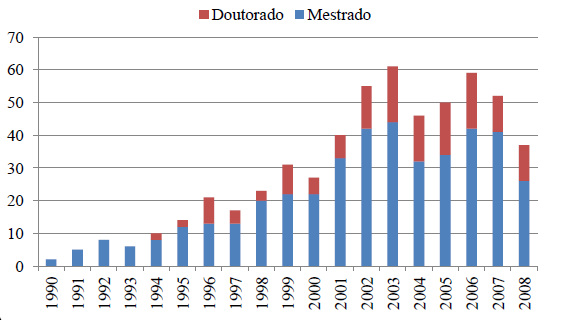
\includegraphics[scale=0.5]{figuras/figura-3}}
	}{
	\Fonte{os autores}
}
\end{figure}

Ou então figuras podem ser incorporadas de arquivos externos, como é o caso da \autoref{fig-grafico-1}. Se a figura que ser incluída se tratar de um diagrama, um gráfico ou uma ilustração que você mesmo produza, priorize o uso de imagens vetoriais no formato PDF. Com isso, o tamanho do arquivo final do trabalho será menor, e as imagens terão uma apresentação melhor, principalmente quando impressas, uma vez que imagens vetorias são perfeitamente escaláveis para qualquer dimensão. Nesse caso, se for utilizar o Microsoft Excel para produzir gráficos, ou o Microsoft Word para produzir ilustrações, exporte-os como PDF e os incorpore ao documento conforme o exemplo abaixo. No entanto, para manter a coerência no uso de software livre (já que você está usando LaTeX e abnTeX),  teste a ferramenta InkScape\index{InkScape}. ao CorelDraw\index{CorelDraw} ou ao Adobe Illustrator\index{Adobe! Illustrator}.  De todo modo, caso não seja possível  utilizar arquivos de imagens como PDF, utilize qualquer outro formato, como JPEG, GIF, BMP, etc.  Nesse caso, você pode tentar aprimorar as imagens incorporadas com o software livre \index{Gimp}Gimp. Ele é uma alternativa livre ao Adobe Photoshop\index{Adobe! Photoshop}.

\section{Usando Fórmulas Matemáticas}

\lipsum[2]

	\begin{equation}
		\begin{aligned}
			x = a_0 + \cfrac{1}{a_1
				+ \cfrac{1}{a_2
					+ \cfrac{1}{a_3 + \cfrac{1}{a_4} } } }
		\end{aligned}
	\end{equation}

\lipsum[3]

	\begin{equation}
		\begin{aligned}
			k_{n+1} = n^2 + k_n^2 - k_{n-1}
		\end{aligned}
	\end{equation}

\lipsum[4]

	\begin{equation}
		\begin{aligned}
			\cos (2\theta) = \cos^2 \theta - \sin^2 \theta
		\end{aligned}
	\end{equation}
	
\lipsum[5]

	\begin{equation}
		\begin{aligned}
			A_{m,n} =
			\begin{pmatrix}
			a_{1,1} & a_{1,2} & \cdots & a_{1,n} \\
			a_{2,1} & a_{2,2} & \cdots & a_{2,n} \\
			\vdots  & \vdots  & \ddots & \vdots  \\
			a_{m,1} & a_{m,2} & \cdots & a_{m,n}
			\end{pmatrix}
		\end{aligned}
	\end{equation}

\lipsum[6]

	\begin{equation}
		\begin{aligned}
			f(n) = \left\{ 
			\begin{array}{l l}
			n/2 & \quad \text{if $n$ is even}\\
			-(n+1)/2 & \quad \text{if $n$ is odd}
			\end{array} \right.
		\end{aligned}
	\end{equation}
	
\lipsum[7]

\section{Usando Algoritmos}

\lipsum[8]

\begin{algorithm}[h!]
	\SetSpacedAlgorithm
	\caption{\label{alg:algoritmo_de_colonica_de_formigas}Algoritmo de Otimização por Colônia de Formiga}
	\Entrada{Entrada do Algoritmo}
	\Saida{Saida do Algoritmo}
	\Inicio{
		Atribua os valores dos parâmetros\;
		Inicialize as trilhas de feromônios\;
		\Enqto{não atingir o critério de parada}{
			\Para{cada formiga}{
				Construa as Soluções\;
			}
			Aplique Busca Local (Opcional)\;
			Atualize o Feromônio\;
		}	
	}		
\end{algorithm}

\lipsum[9]

\section{Usando Código-fonte}

\lipsum[10]

\lstinputlisting[language=C++,caption={Hello World em C++}]{figuras/main.cpp}

\lipsum[11]

\begin{lstlisting}[language=Java,caption={Hello World em Java}]
public class HelloWorld {
	public static void main(String[] args) {
		System.out.println("Hello World!");
	}
}
\end{lstlisting}

\lipsum[11]

\section{Usando Teoremas, Proposições, etc}

Lorem ipsum dolor sit amet, consectetur adipiscing elit. Nunc dictum sed tortor nec viverra. consectetur adipiscing elit. Nunc dictum sed tortor nec viverra.

\begin{teo}[Pitágoras]
	Em todo triângulo retângulo o quadrado do comprimento da
	hipotenusa é igual a soma dos quadrados dos comprimentos dos catetos.
\end{teo}


Lorem ipsum dolor sit amet, consectetur adipiscing elit. Nunc dictum sed tortor nec viverra. consectetur adipiscing elit. Nunc dictum sed tortor nec viverra.

\begin{teo}[Fermat]
	Não existem inteiros $n > 2$, e $x, y, z$ tais que $x^n + y^n = z$
\end{teo}

Lorem ipsum dolor sit amet, consectetur adipiscing elit. Nunc dictum sed tortor nec viverra. consectetur adipiscing elit. Nunc dictum sed tortor nec viverra.

\begin{prop}
	Para demonstrar o Teorema de Pitágoras...
\end{prop}

Lorem ipsum dolor sit amet, consectetur adipiscing elit. Nunc dictum sed tortor nec viverra. consectetur adipiscing elit. Nunc dictum sed tortor nec viverra.

\begin{exem}
	Este é um exemplo do uso do ambiente exe definido acima.
\end{exem}

Lorem ipsum dolor sit amet, consectetur adipiscing elit. Nunc dictum sed tortor nec viverra. consectetur adipiscing elit. Nunc dictum sed tortor nec viverra.

\begin{xdefinicao}
	Definimos o produto de ...
\end{xdefinicao}

Lorem ipsum dolor sit amet, consectetur adipiscing elit. Nunc dictum sed tortor nec viverra. consectetur adipiscing elit. Nunc dictum sed tortor nec viverra.

\section{Usando Questões}


Lorem ipsum dolor sit amet, consectetur adipiscing elit. Nunc dictum sed tortor nec viverra. consectetur adipiscing elit. Nunc dictum sed tortor nec viverra.

\begin{questao}
	\item Esta é a primeira questão com alguns itens:
		\begin{enumerate}
			\item Este é o primeiro item
			\item Segundo item
		\end{enumerate}
	\item Esta é a segunda questão:
		\begin{enumerate}
			\item Este é o primeiro item
			\item Segundo item
		\end{enumerate}
	\item Lorem ipsum dolor sit amet, consectetur adipiscing elit. Nunc dictum sed tortor nec viverra. consectetur adipiscing elit. Nunc dictum sed tortor nec viverra.
		\begin{enumerate}
			\item consectetur
			\item adipiscing
			\item Nunc
			\item dictum
		\end{enumerate}
\end{questao}

\section{Citações}

\subsection{Documentos com três autores}

Quando houver três autores na citação, apresentam se os três, separados por ponto e vírgula, caso estes estejam após o texto. Se os autores estiverem incluídos no texto, devem ser separados por vírgula e pela conjunção "e".

\citeautoronline{tresautores}

\cite{tresautores}

\subsection{Documentos com mais de três autores}
Havendo mais de três autores, indica-se o primeiro seguido da expressão \textit{et al.} (do latim \textit{et alli}, que significa e outros), do ano e da página.

\citeautoronline{quatroautores}

\cite{quatroautores}

\cite{kurose2013}

\cite{pinheiro2004site}

\cite{costa1998}

\cite{gorshe2014ieee}

\citeautoronline{cartilhaUCAredessemfio}

\cite{moraes2014}

\cite{amer2016acm}

\cite{tanenbaum2013}

\cite{rodrigues2007site}

\cite{marconi2017}

\cite{gil2002}

\cite{barbosa2012}

\cite{wiki}

\subsection{Documentos de vários autores}

Havendo    citações    indiretas de    diversos    documentos    de    vários    autores, mencionados  simultaneamente e  que  expressam  a  mesma  ideia,  separam-se  os  autores  por ponto e vírgula, em ordem alfabética.

\cite{tresautores, quatroautores}

\section{Notas de Rodap\'{e}}

%Deve-se utilizar o sistema autor-data para as  citações no texto e o numérico para notas explicativas\footnote{Veja - se como exemplo desse tipo de abordagem o estudo de Netzer (1976)}. As notas de rodapé podem e devem ser alinhadas, a partir da segunda linha da mesma nota, abaixo da primeira letra da primeira palavra, de forma a destacar o expoente \footnote{Encontramos  esse  tipo  de  perspectiva  na  2ª  parte  do  verbete  referido  na  nota  anterior,  em  grande  parte  do estudo de Rahner (1962).} e sem espaço entre elas e com fonte menor (tamanho 10).


	\chapter{Resultados}
\label{chap:resultados}

\lipsum[2]

\section{Resultados do Experimento A}
\label{sec:resultados-do-experimento-a}

\lipsum[3]

\section{Resultados do Experimento B}
\label{sec:resultados-do-experimento-b}

\lipsum[4]
	\chapter{Conclusões e Trabalhos Futuros}
\label{chap:conclusoes-e-trabalhos-futuros}

\lipsum[2]
\lipsum[34]

\section{Contribuições do Trabalho}
\label{sec:contribuicoes-do-trabalho}

\lipsum[3]

\section{Limitações}
\label{sec:limitacoes}

\lipsum[4]

\section{Trabalhos Futuros}
\label{sec:trabalhos-futuros}

\lipsum[5]





	
	% Meu TCC
	\chapter{Introdução}
\label{cap:introducao}

\section{Contextualização}
\label{sec:contextualizacao}

Na década de 1970, o sistema Aloha\footnote{Originalmente, o sistema Aloha, desenvolvido por Norman Abramson em 1970, na Universidade do Havaí, funcionava como um protocolo para sistemas de comunicação via radiofrequência para o acesso remoto entre computadores enviando pacotes num sistema de radiocomunicação \cite{abramson1970acm,haykin2008}.} estabeleceu e operou uma rede de dados terrestres (AlohaNet) no estado americano do Havaí. O sistema usou um transponder acoplado em um satélite experimental da Agência Espacial Americana (NASA, do inglês, \textit{National Aeronautics and Space Administration}) (ATS-1) para demonstrar uma rede internacional de dados via satélite conectando a NASA, na Califórnia, e cinco universidades nos Estados Unidos, Japão e Austrália, fornecendo a primeira demonstração pública de uma rede de dados por pacotes sem fio \cite{abramson1970acm,SchwartzAbramson2009ieee}.

Mesmo com limitações como largura de banda e tecnologia de transmissão, foi graças ao pioneirismo do sistema Aloha, que as redes de comutação sem fio locais, conhecidas como LANs (do inglês, \textit{Local Area Network}) sem fio ou ainda WLANs (do inglês, \textit{Wireless Local Area Network}) surgiram como redes complementares às redes cabeadas tradicionais. Essa tecnologia de comunicação se desenvolveu devido a necessidade de implementação de um método alternativo de conexão que não privasse a movimentação do usuário durante a conexão com a rede. O tempo passou e a tecnologia evoluiu, deixou de ser restrita ao meio acadêmico e militar e se tornou acessível a empresas e ao usuário doméstico. Nos dias de hoje se pode pensar em redes \textit{wireless} (``sem fio'', em português) como uma alternativa bastante interessante em relação às redes cabeadas. Suas aplicações são muitas e variadas e o fato de ter a mobilidade como principal característica, tem facilitado a sua aceitação, principalmente nas empresas \cite{farias2005}.

Com o advento de \textit{notebooks}, \textit{tablets}, \textit{smartphones} e a promessa de acesso desimpedido à Internet global de qualquer hora e lugar por meio das comunicações sem fio, a demanda de acesso de dispositivos sem fio à Internet aumentou consideravelmente não só através da rede de telefonia móvel, agora plenamente possível, mas também por meio das redes Wi-Fi (do inglês, \textit{Wireless Fidelity}). O uso deste tipo de rede está se tornando cada vez mais comum, não só nos ambientes domésticos e corporativos, mas também em locais públicos (bares, lanchonetes, \textit{shoppings}, aeroportos, etc) e em instituições acadêmicas. Independentemente do crescimento futuro de equipamentos sem fio para Internet, já ficou claro que as redes sem fio e os serviços móveis relacionados que elas possibilitam se popularizaram e fazem parte do cotidiano das pessoas \cite{gast2002,kurose2013}.

Esse crescimento se deu, principalmente, com os avanços tecnológicos feitos na área, tornando a conexão mais rápida e confiável na troca de dados entre os nós da rede, fazendo com que os dispositivos móveis agregassem praticamente todas as funções que teria um computador de mesa convencional. Como consequência, estima-se que a força de trabalho móvel, em 2020, corresponderá a aproximadamente 1,75 bilhão de trabalhadores, segundo a Organização Internacional do Trabalho \cite{wba2017}. Para estes bilhões de usuários móveis, trabalhando dentro e fora do escritório tradicional, a mobilidade se tornou sinônimo de produtividade.

\textcolor{blue}{Segundo \citeonline{wba2017}, quando se trata de conexão sem fio com a Internet, os trabalhadores móveis preferem redes Wi-Fi ao invés de redes celulares, que são mais caras. Dessa forma, o Wi-Fi transporta mais da metade de todos os dados móveis de acordo com o Índice de Rede Visual da Cisco (VNI, do inglês, \textit{Visual Networking Index}) \cite{wba2017}.}

\section{Justificativa}
\label{sec:justificativa}

\textcolor{blue}{Os sistemas de telecomunicação utilizam cada vez mais as tecnologias sem fio.} Como resultado, as formas tradicionais de trabalho em rede no mundo mostraram-se inadequadas para enfrentar os desafios apresentados por nosso novo estilo de vida coletivo. Se os usuários precisarem estar conectados a uma rede por cabos físicos, seu movimento será drasticamente reduzido. A conectividade sem fio, no entanto, não apresenta esta restrição e permite muito mais movimento livre por parte do usuário da rede. Como consequência, as tecnologias sem fio estão invadindo o domínio tradicional das redes ``fixas'' ou ``com fio'' \cite{gast2002}.

As redes sem fio compartilham várias vantagens importantes. A vantagem mais evidente da rede sem fio é a mobilidade. Usuários de redes sem fio podem se conectar às redes existentes e, em seguida, podem circular livremente. Por exemplo, um usuário de telefone celular pode percorrer quilômetros no decorrer de uma única conversa desde que ele esteja coberto por alguma torre celular \cite{gast2002}.

%Da mesma forma, as redes Wi-Fi liberam os desenvolvedores de \textit{software} das amarras de um cabo Ethernet em uma mesa. Os desenvolvedores podem trabalhar na biblioteca, em uma sala de conferências, no estacionamento ou até mesmo na lanchonete do outro lado da rua. Enquanto os usuários sem fio permanecerem dentro do alcance do equipamento transmissor, eles poderão tirar proveito da rede \cite{gast2002}.

Em escolas e universidades, os laboratórios e bibliotecas estão quase sempre repletos de alunos que encontram na rede (Internet) uma boa fonte de consultas e pesquisas que complementam o conteúdo abordado em sala de aula, além de facilitar a comunicação e a troca de informações entre os estudantes. Graças à tecnologia de comunicação sem fio Wi-Fi, estudantes e professores não dependem exclusivamente dos laboratórios de informática para se conectarem à Internet.

O acesso sem fio pode ser disponibilizado por todo o ambiente educacional, bastando apenas o usuário ligar seu \textit{notebook} ou dispositivo móvel de qualquer local com cobertura e estabelecer a conexão com a rede.

%Outra propriedade benéfica das redes sem fio é que estas geralmente têm muita flexibilidade, o que pode se traduzir em implantação rápida. Redes sem fio usam um número de estações base para conectar usuários a uma rede existente. O lado da infraestrutura de uma rede sem fio, no entanto, é qualitativamente o mesmo, esteja conectando um usuário ou um milhão de usuários. Para oferecer serviço em uma determinada área, é necessário a presença de estações base e antenas no lugar.

%Uma vez que essa infraestrutura é construída, adicionar um usuário a uma rede sem fio é principalmente uma questão de autorização. Com a infraestrutura disponível, ela deve ser configurada para reconhecer e oferecer serviços aos novos usuários, mas a autorização não exige mais infraestrutura. Adicionar um usuário a uma rede sem fio é uma questão de configurar a infraestrutura, mas isso não envolve a passagem de cabos, o fechamento de terminais e a aplicação de correções em um conector \cite{gast2002}.

%Este exemplo simples ignora os desafios de escalabilidade. Naturalmente, se os novos usuários sobrecarregarem a infraestrutura existente, a própria infraestrutura precisará ser reforçada para que mais usuários possam ser conectados. A expansão da infraestrutura pode ser cara e demorada, especialmente se envolver aprovação legal e regulatória de faixas de frequência. No entanto, o ponto básico é válido: adicionar um usuário a uma rede sem fio pode ser reduzido a uma questão de configuração, enquanto adicionar um usuário a uma rede fixa requer conexões físicas \cite{gast2002}.

%Embora seja possível atender a um grupo fluido de usuários com conectores padrão Ethernet, o fornecimento de acesso através de uma rede com fio é problemático por vários motivos. A passagem de cabos é demorada, cara e também pode exigir adaptações no espaço físico; determinar corretamente o número de enlaces de cabos é difícil devido ao intenso fluxo de pessoas. Com uma rede sem fio, porém, não há necessidade de eventuais alterações na construção ou fazer suposições estatísticas complexas sobre a demanda. Uma infraestrutura com fio simples se conecta à Internet e, em seguida, a rede sem fio pode acomodar quantos usuários forem necessários \cite{gast2002}.

%Apesar das várias vantagens oferecidas pelas redes sem fio, as mesmas não substituem as LANs cabeadas. Servidores e outros equipamentos de \textit{datacenter} devem acessar dados, mas a localização geográfica do servidor é irrelevante. A velocidade das redes sem fio é limitada pela largura de banda disponível. A teoria da informação pode ser usada para deduzir o limite da velocidade de uma rede. A menos que as autoridades reguladoras estejam dispostas a aumentar as bandas de espectro não licenciadas, há um limite superior na velocidade das redes sem fio. O \textit{hardware} de rede sem fio tende a ser mais lento que o \textit{hardware} com fio. Diferentemente do padrão Ethernet, os padrões de rede sem fio devem avaliar cuidadosamente os quadros de entrada para proteger contra perda devido à falta de confiabilidade do meio \textit{wireless} \cite{gast2002}.

Para quantificar a relevância das redes \textit{wireless}, em 2022, 51\% do tráfego de dados móveis global será transportado pela redes Wi-Fi segundo a Cisco VNI no ano de 2018. No Brasil, 48\% do tráfego de dados total da Internet será movido através das redes Wi-Fi de acordo com as estimativas disponibilizadas também pela Cisco VNI em 2018.

Para que haja transferência de dados, as redes sem fio usam ondas de rádio como meio de transmissão, entretanto essa abordagem apresenta vários desafios. As ondas de rádio podem sofrer vários problemas de propagação que podem interromper o \textit{link} de rádio, como interferência, perdas de multipercurso e áreas de sombra (locais sem cobertura de sinal), que podem atenuar a potência do sinal Wi-Fi, reduzindo, por consequência, a taxa de transferência e a qualidade da conexão, assim como a viabilidade de alguns serviços que exigem um limite mínimo destes recursos para funcionar com eficiência
 \cite{gast2002}. Isso significa que o canal de rádio impõe limitações fundamentais para o desempenho dos sistemas de comunicação sem fio.
 
Devido ao amplo crescimento e ao alto interesse pela criação de ambientes com mobilidade no acesso à rede em instituições públicas e também no mercado privado, torna-se essencial um estudo aprofundado na área ao planejar ou avaliar novas instalações, sempre buscando qualidade, confiabilidade e respeito às normas técnicas e legislação vigente.

% Proposta do trabalho
Para que uma WLAN tenha um desempenho satisfatório aos seus usuários, vários fatores devem ser levados em consideração para que o processo de instalação corresponda o mais fielmente possível ao planejado. Um método amplamente utilizado por projetista de redes, seja cabeada ou sem fio, é o \textit{site survey}. O \textit{site survey} é um conjunto de métodos de análise detalhada da estrutura do local onde será implantada a nova rede ou aplicada a uma infraestrutura já existente com o objetivo de identificar e solucionar problemas no sistema \cite{pinheiro2004site}.

Portanto, a proposta deste trabalho consiste em analisar a infraestrutura geral da rede sem fio do Bloco Didático do IFCE \textit{campus} Tauá a fim de avaliar se a configuração atual da rede sem fio provê um serviço satisfatório baseado na análise dos mapas de calor dos sinais de rádio da área.

Mediante o exposto, nesta proposta de trabalho será empregado a técnica de projeto chamada \textit{site survey} para levantar dados do Bloco Didático, especialmente sobre como ocorre a propagação dos sinais e medir o nível de sinal da rede sem fio, a partir dos pontos de acesso já presentes no local, pois estes são aspectos de grande impacto no desempenho das redes sem fio em geral.  Este método tem como intuito detectar possíveis problemas que incapacite a rede de prover a cobertura necessária para que serviços básicos (pesquisas, estudos, experimentos, etc.) dos estudantes, docentes e servidores sejam atendidas com o mínimo de satisfação.

É extremamente recomendado aliar ao \textit{site survey} ferramentas complementares para auxiliar o processo de inspeção do local, como, por exemplo, um \textit{software} adequado instalado em um \textit{notebook} que possa realizar a medição de potência do sinal e também identificar o canal de frequência em que opera as redes vizinhas, com objetivo de identificar possíveis interferências destrutivas no sinal.

Depois de fazer uso da ferramenta apropriada para a análise, é importante identificar o ambiente de trabalho para determinar a localização dos equipamentos e analisar o desempenho da rede Wi-Fi, para garantir uma melhor cobertura e prestar um melhor serviço.

Com os resultados se buscará simular o grau de eficiência da infraestrutura de rede sem fio ofertada pelo IFCE Tauá ao Bloco Didático, propor uma solução para conseguir um melhor desempenho através de recomendações para otimizar o serviço de rede \textit{wireless}.

\section{Objetivos}
\label{sec:objetivos}

Este trabalho apresenta como objetivo geral mostrar a aplicação da metodologia \textit{site survey} para análise de cobertura e recepção do sinal Wi-Fi no Bloco Didático do Instituto Federal do Ceará \textit{campus} Tauá.
Já com relação aos objetivos específicos, este trabalho visa:
\begin{compactitem}
	\item Analisar a infraestrutura atual da rede sem fio do Bloco Didático através de sua planta estrutural;
	\item Identificar e localizar os locais de concentração dos pontos de acesso para a elaboração de plantas, desenhos ou esquemáticos;
	\item Verificar a presença de possíveis obstáculos, fontes de interferência e áreas de sombra que possam limitar a propagação do sinal da rede sem fio;
	\item Coletar dados em campo do Bloco Didático a respeito da propagação do sinal da rede Wi-Fi;
	\item Sugerir uma melhoria para a rede com base nos resultados obtidos.
\end{compactitem}

\section{Organização do Trabalho}
\label{sec:organnizacao-do-trabalho}

Este trabalho está dividido da seguinte forma:

\begin{compactitem}
	\item Capítulo 2: aborda os principais conceitos por trás do processo de transmissão em redes sem fio, essenciais para a compreensão do funcionamento geral das comunicações sem fio, incluindo os mecanismos básicos da propagação de ondas eletromagnéticas e alguns modelos de propagação utilizados na predição de enlaces de rádio, tanto para ambientes internos quanto para ambientes externos.
	
	\item Capítulo 3: apresenta as principais características das redes Wi-Fi, a sua arquitetura, o padrão IEEE 802.11 (o qual as redes Wi-Fi são estruturadas) e, por fim, o método de inspeção \textit{site survey} como ferramenta para o planejamento e avaliação de redes \textit{wireless}.
	
	\item Capítulo 4: apresenta um estudo de caso realizado a partir da aplicação do \textit{site survey} na infraestrutura de rede sem fio do Bloco Didático do Instituto Federal de Educação, Ciência e Tecnologia do Ceará \textit{campus} Tauá; Expõe e discute os resultados obtidos ao fim do processo de coleta de dados do local alvo; Propõe medidas de intervenção na infraestrutura da rede para a melhoria da cobertura do sinal nos dois andares analisados.
	
	\item Capítulo 5: apresenta o encerramento do trabalho baseado no conteúdo discutido e nos resultados obtidos no estudo de caso.
\end{compactitem}
	\chapter{Transmissão em Redes sem Fio}
\label{cap:transmissao-redes-sem-fio}

\section{O Espectro Eletromagnético}
\label{sec:espectro-eletromagnetico}

Quando se movem, os elétrons criam ondas eletromagnéticas que podem se propagar pelo espaço livre (até mesmo no vácuo), transportando energia durante o percurso. Essas ondas foram previstas pelo físico inglês James Clerk Maxwell em 1865 e foram observadas pela primeira vez pelo físico alemão Heinrich Hertz em 1887 \cite{tanenbaum2011}. O número de ciclos (oscilações) por segundo de uma onda eletromagnética é chamado frequência, e é medido em Hertz (Hz) -- em homenagem a Heinrich Hertz. A distância entre dois pontos máximos (ou mínimos) consecutivos é chamada comprimento de onda, designada universalmente pela letra grega $\lambda$ (lambda).

A velocidade de uma onda qualquer depende do meio em que ela se propaga. No vácuo, todas as ondas eletromagnéticas viajam na mesma velocidade, a da luz, que é aproximadamente igual a $3 \times 10^8$ m/s, independentemente de sua frequência \cite{tanenbaum2011}.

Essas três grandezas -- frequência ($f$), comprimento de onda ($\lambda$) e velocidade ($c$) -- se relacionam (no vácuo) através da seguinte expressão:
\begin{equation}
	\begin{aligned}
		c = \lambda f
	\end{aligned}
\end{equation}
\begin{figure}[H]
	\centering
	\Caption{\label{fig:onda}Propriedades de uma onda.}	
	\UECEfig{}{
		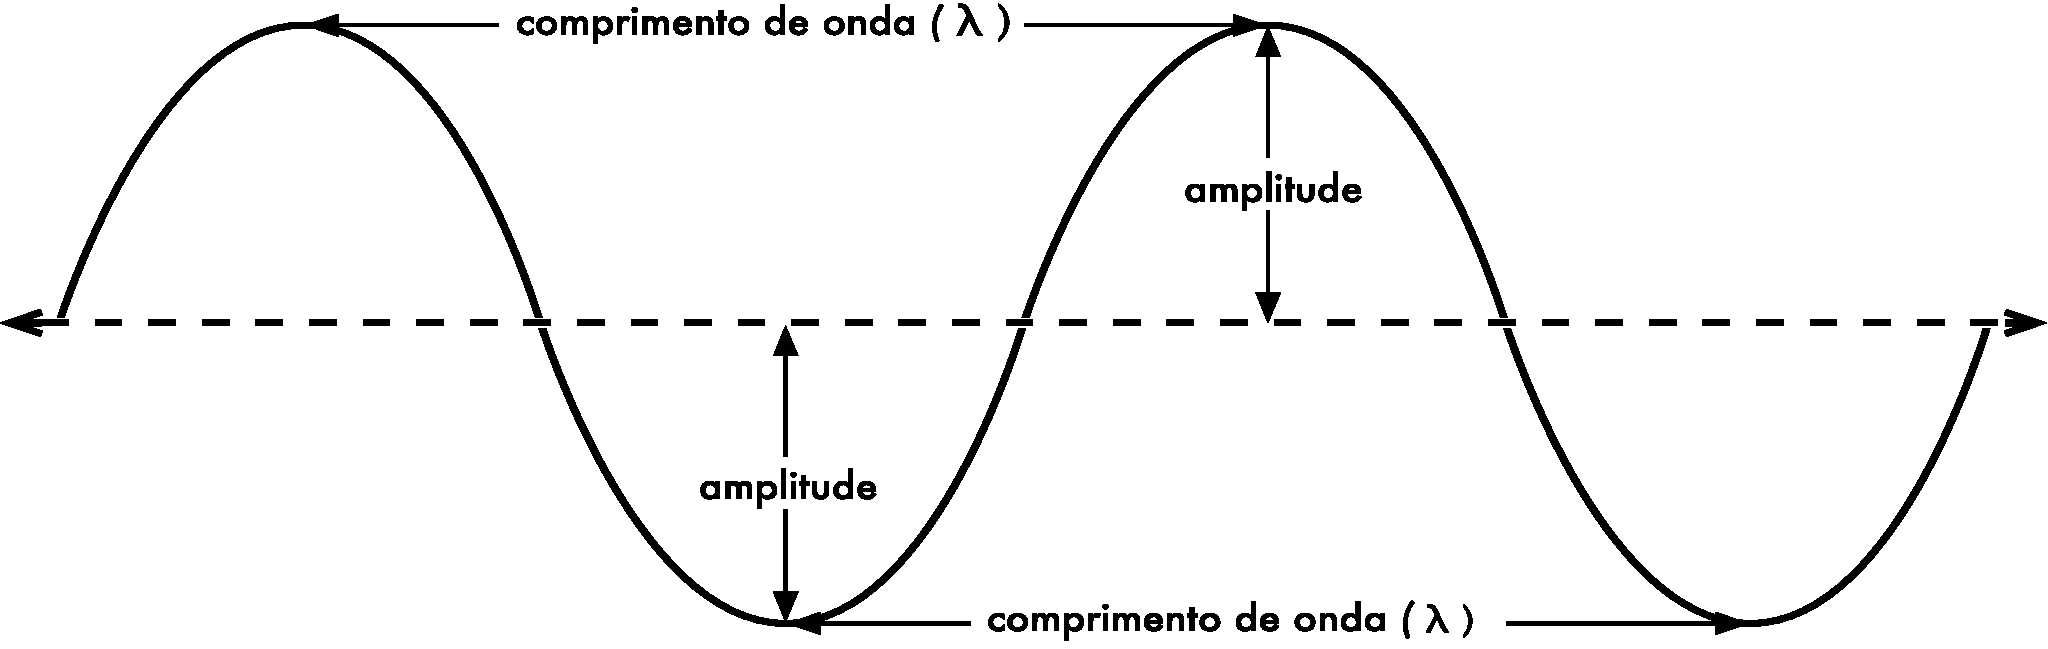
\includegraphics[scale=.4]{figuras/onda0.pdf}
	}{
		\Fonte{\citeonline[p. ~10]{flickenger2008}.}
	}	
\end{figure}

Uma vantagem da onda eletromagnética é o fato de que ela pode ser gerada ou captada por circuitos eletrônicos simples. Além disso, esse tipo de onda se propaga no vácuo, o que permite a comunicação entre antenas terrestres com satélites no espaço e vice-versa, entre os próprios satélites e entre dois pontos localizados em qualquer parte da superfície terrestre \cite{fluminense2010}.

Os dispositivos sem fio são restritos para operar em uma determinada banda (ou faixa) de frequência. Cada faixa tem uma largura de banda associada, que é simplesmente a quantidade de espaço de frequência na banda. Se a variação entre 2,40 GHz e 2,48 GHz é usada por um dispositivo, então a largura de banda será de 0,08 GHz ou 80 MHz.

A largura de banda adquiriu uma conotação de ser uma medida da capacidade de dados de um \textit{link}. Uma grande quantidade de matemática, teoria da informação e processamento de sinais pode ser usada para demonstrar que fatias mais largas de frequência podem ser usadas para transmitir mais informações \cite{gast2002}. Por exemplo, um canal de telefonia móvel analógico requer uma largura de banda de 20 kHz. Os sinais de televisão são muito mais complexos, já que, necessariamente, transmitem tráfego de áudio e vídeo, e por esse motivo possuem uma largura de banda consideravelmente maior, cerca de 6 MHz \cite{gast2002}.

O uso de uma faixa de frequência é rigorosamente controlado pelas autoridades reguladoras através de processos de licenciamento. No âmbito mundial, o processo de padronização de alocação de frequências para uso específico é realizado pela União Internacional de Telecomunicações (ITU, do inglês, \textit{International Telecommunication Union}). No Brasil, a ANATEL (Agência Nacional de Telecomunicações) representa a entidade responsável pela definição e fiscalização da utilização das faixas de frequência em território nacional. Essas determinações regulatórias visam coibir o uso das faixas de frequência sem permissão por infratores como estações de rádio e TVs piratas.

Entretanto, existem faixas de frequência que não estão sujeitas a autorização de uso pelos órgãos reguladores, ou seja, são bandas de frequência abertas para transmitir. Essas frequências não licenciadas são conhecidas como ISM (do inglês, \textit{Industrial, Scientific, Medical}). As bandas ISM foram padronizadas na maioria dos países em três faixas de frequência: 900 MHz, 2,4 GHz e 5 GHz \cite{moraes2010,tanenbaum2011}. A figura abaixo exibe a alocação das frequências ISM e também das bandas U-NII (do inglês, \textit{Unlicensed National Information Infrastructure}).
\begin{figure}[H]
	\centering
	\Caption{\label{fig:ism_unii}As bandas ISM e U-NII.}	
	\UECEfig{}{
		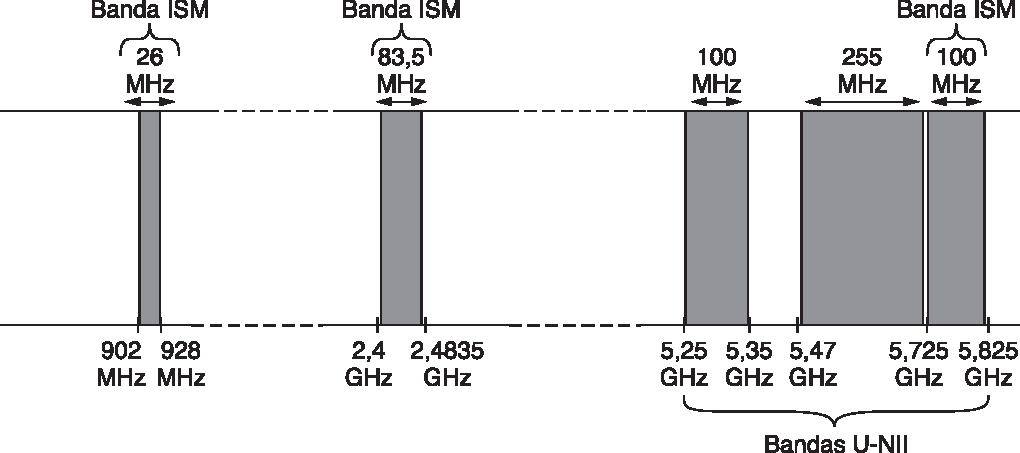
\includegraphics[scale=.6]{figuras/ism-unii.pdf}
	}{
		\Fonte{\citeonline[p. ~66]{tanenbaum2011}.}
	}	
\end{figure}

Cada banda de frequência utilizada nas telecomunicações estão contidas em um modelo de escala comum, onde é apresentado o intervalo completo de todas as possíveis frequências da radiação eletromagnética, denominado de espectro eletromagnético. A figura abaixo ilustra todas as variações de frequências contidas no espectro eletromagnético.
\begin{figure}[H]
	\centering
	\Caption{\label{fig:espectro}O espectro eletromagnético e a maneira como ele é usado na comunicação.}	
	\UECEfig{}{
		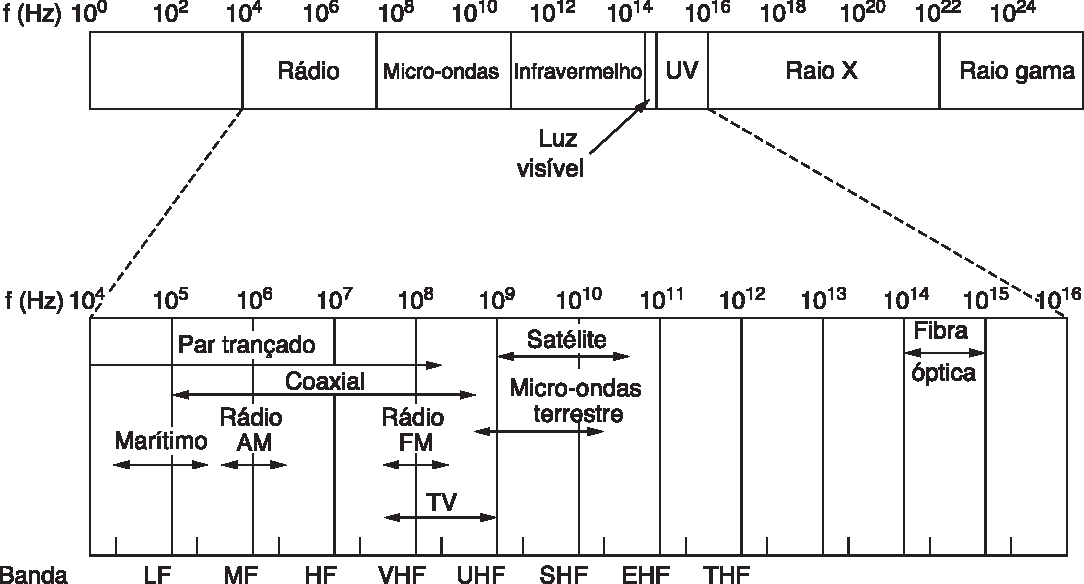
\includegraphics[scale=.72]{figuras/espectro_eletromagnetico.pdf}
	}{
		\Fonte{\citeonline[p. ~70]{tanenbaum2011}.}
	}	
\end{figure}

\begin{citacao}
	As faixas de rádio, microondas, infravermelho e luz visível do espectro podem ser usadas na transmissão de informações, por meio de modulação da amplitude, da frequência ou da fase das ondas. A luz ultravioleta, os raios X e os raios gama representariam opções ainda melhores, por terem frequências mais altas, mas são difíceis de produzir e modular, além de não se propagarem bem através dos prédios e de serem perigosos para os seres vivos \cite{tanenbaum2011}.
\end{citacao}

\section{Efeitos de Propagação em Ondas Eletromagnéticas}
\label{sec:efeitos-propagacao-OE}

Sistemas de comunicações sem fio utilizam-se de ondas eletromagnéticas para o envio de sinais através do ar. Na perspectiva de um usuário, conexões sem fio não são particularmente diferentes de qualquer outro tipo de conexão de rede: os serviços de transmissão de informações funcionarão de acordo com o esperado \cite{flickenger2008}. Mas ondas de rádio possuem algumas propriedades inesperadas se comparadas com o meio guiado.  Por exemplo: é muito fácil ver o caminho que o cabo Ethernet faz, só é preciso seguí-lo em sua extensão. Também pode-se ter a confiança de que ter vários cabos Ethernet lado a lado não causarão problemas, uma vez que os sinais trafegam no interior dos fios.

Diferentemente dos enlaces físicos, o caminho de uma onda de rádio entre transmissor e receptor pode variar de uma simples linha de visão completamente desobstruída até um cenário em que seja obstruído por prédios, terrenos elevados e áreas de vegetação densa \cite{rappaport2009}. Isso quer dizer que os sinais de rádio são aleatórios e de difícil análise. Até a velocidade do deslocamento dos terminais influencia na rapidez com que o sinal enfraquece \cite{rappaport2009}.

Portanto, o estudo da propagação dos sinais de radiofrequência é importante para a compreensão das comunicações sem fio porque fornece a modelagem física necessária, o que resulta em uma boa estimativa de potência requerida para o estabelecimento do enlace de comunicação para que haja comunicação confiável \cite{haykin2008}. Além disso, o estudo da propagação auxilia na compreensão das técnicas de recepção para compensação das perdas introduzidas pela transmissão sem fio \cite{haykin2008}.

Os efeitos sofridos pela onda eletromagnética ao se propagar são diversos, mas os principais e mais importantes são a reflexão, a difração, a refração, a absorção, o desvanecimento e a interferência \cite{flickenger2008,haykin2008,rappaport2009}.

\subsection{Absorção}
\label{sub:absorcao}

Quando ondas eletromagnéticas penetram algum objeto, elas geralmente atenuam ou dissipam-se totalmente. O quanto elas perdem de potência irá depender de sua frequência e, claro, do material em que penetram \cite{flickenger2008}. Em analogia, janelas de vidro são, obviamente, transparentes para a luz, enquanto o vidro usado em óculos de sol filtram uma boa quantidade da intensidade da luz e também da radiação ultravioleta.
\begin{figure}[H]
	\centering
	\Caption{\label{fig:absorcao}Atenuação devido a absorção.}	
	\UECEfig{}{
		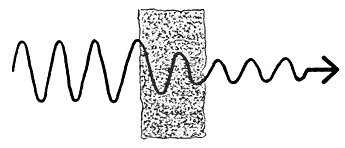
\includegraphics[scale=.74]{figuras/absorcao1.png}
	}{
		\Fonte{Adaptado de \citeonline{megasorber2019c}.}
	}
\end{figure}

Para ondas de rádio, os dois principais materiais absorventes são \cite{flickenger2008}:

\begin{alineascomnumero}
	\item Metal: elétrons podem mover-se livremente em metais, sendo prontamente capazes de oscilar e absorver a energia de uma onda que incida sobre eles;
	\item Água: ondas de rádio fazem com que as moléculas de água agitem-se, tomando parte da energia da onda.
\end{alineascomnumero}

Em termos práticos de redes sem fio, podemos considerar os metais e a água como excelentes absorventes: as ondas de rádio não serão capazes de atravessá-los com facilidade \cite{flickenger2008}.

\subsection{Reflexão}
\label{sub:reflexao}

Nas comunicações sem fio terrestres, normalmente não existe uma linha de visada desimpedida no percurso do sinal de rádio entre transmissor e receptor e as comunicações geralmente envolvem o fenômeno da reflexão \cite{haykin2008}.

\begin{citacao}
	A reflexão ocorre quando uma onda eletromagnética em propagação colide com um objeto que possui dimensões muito grandes em comparação com o comprimento de onda da onda que se propaga  \cite{rappaport2009}.
\end{citacao}

\begin{figure}[H]
	\centering
	\Caption{\label{fig:reflexao}Reflexão.}	
	\UECEfig{}{
		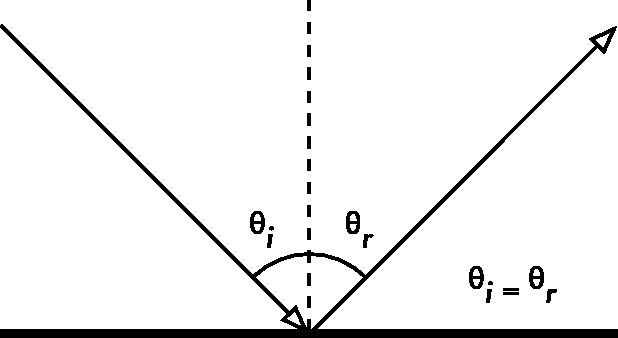
\includegraphics[scale=.65]{figuras/reflexao.pdf}
	}{
		\Fonte{\citeonline[p. ~18]{flickenger2008}.}
	}
\end{figure}

\subsubsection{Multipercurso}
\label{subsec:multipercurso}

Ainda que as regras de reflexão sejam relativamente simples, a situação pode se complicar quando se imagina o interior de um escritório com várias divisórias e objetos metálicos das mais variadas formas e tamanhos. O mesmo se aplica aos ambientes urbanos, já que estes apresentam construções de concreto, árvores, veículos e um intenso fluxo de pessoas circulando pelas ruas.

Nessas áreas densamente ocupadas, a maior parte da comunicação acontece por espalhamento das ondas eletromagnéticas ao chocarem-se contra a superfície das construções e objetos ao redor \cite{haykin2008}.  Esses percursos de propagação múltiplos são conhecidos como multipercurso ou multicaminho. Até mesmo quando existe uma linha de visão direta, o multipercurso ainda ocorre devido às reflexões no solo e nas estruturas próximas a estação móvel \cite{rappaport2009}.
\begin{figure}[H]
	\centering
	\Caption{\label{fig:multipath}Sinais refletidos.}	
	\UECEfig{}{
		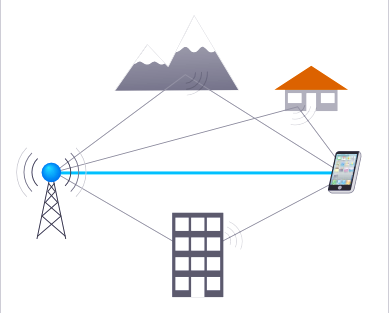
\includegraphics[scale=.8]{figuras/Multipath1.png}
	}{
		\Fonte{Adaptado de \citeonline{yatebts2015}.}
	}
\end{figure}

\subsection{Difração}
\label{sub:difracao}

\begin{citacao}
	A difração ocorre quando o caminho de rádio entre o transmissor e o receptor é obstruído por uma superfície que possui irregularidades afiadas (arestas). As ondas secundárias resultantes da superfície de obstrução estão presentes pelo espaço e até mesmo por trás do obstáculo, fazendo surgir uma curvatura de ondas em torno do obstáculo, até mesmo quando não existe um caminho de linha de visão entre transmissor e receptor \cite{rappaport2009}.
\end{citacao}

O fenômeno da difração, de maneira sucinta, está relacionado ao fato de as ondas eletromagnéticas contornarem objetos quando passam ao redor dos mesmos, tais como arestas de construções ou picos de montanhas ou quando atravessam barreiras contendo aberturas. Para altas frequências, a difração, assim como a reflexão, depende do formato do objeto, além da amplitude, fase e polarização da onda incidente sobre o ponto difrator \cite{rappaport2009}.
\begin{figure}[H]
	\centering
	\Caption{\label{fig:difracao}Difração sobre o topo de uma montanha.}	
	\UECEfig{}{
		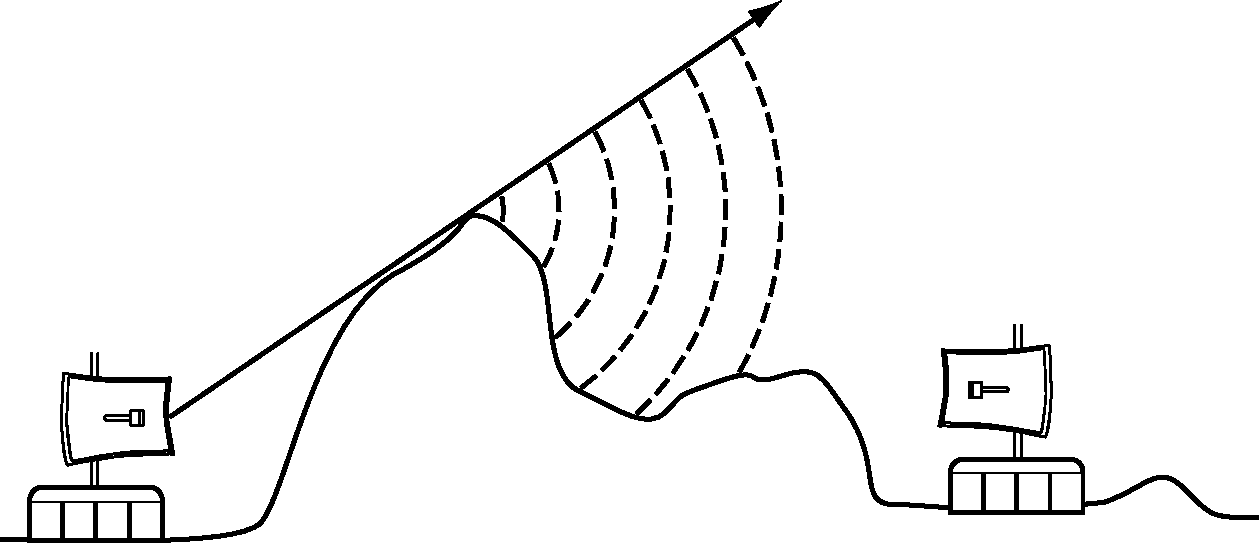
\includegraphics[scale=.6]{figuras/difracao1.pdf}
	}{
		\Fonte{\citeonline[p. ~20]{flickenger2008}.}
	}
\end{figure}

Vale ressaltar que a difração ocorre ao custo de perda de potência, isto é, a energia da onda difratada é significativamente menor que a da onda original. Mas ainda sim existe, nas ondas secundárias, força suficiente para produzir um sinal útil, além da vantagem da difração para contornar obstáculos \cite{flickenger2008,rappaport2009}.

\subsection{Refração}
\label{sub:refracao}

A refração ocorre quando as ondas eletromagnéticas mudam a trajetória de propagação quando passam de um meio para outro. Na transição, o nível de energia da onda é reduzido, pois uma fração da onda é refletida \cite{flickenger2008}. Um exemplo de refração ocorre quando a luz, propagando-se no ar, encontra uma interface com a água. A utilização da refração nas comunicações sem fio fica limitada a circunstâncias especiais, tais como comunicações via satélite, pois a transmissão necessita penetrar através das camadas da atmosfera, cada uma com densidade distinta da outra \cite{rappaport2009}.
\begin{figure}[H]
	\centering
	\Caption{\label{fig:refracao}Refração.}	
	\UECEfig{}{
		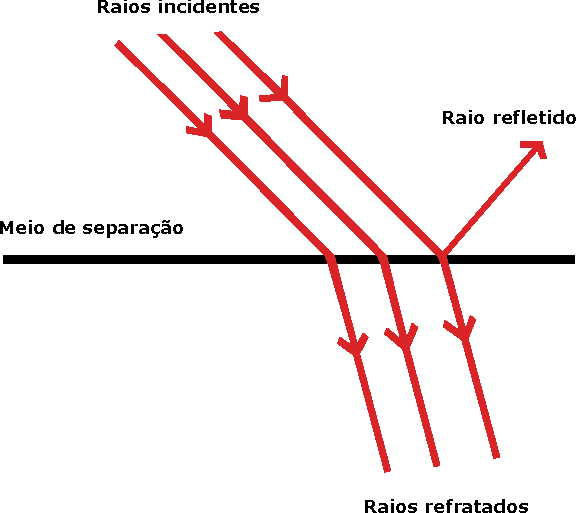
\includegraphics[scale=.68]{figuras/refracao.pdf}
	}{
		\Fonte{Adaptado de \citeonline{teixeira2019c}.}
	}
\end{figure}

\subsection{Interferência}
\label{sub:interferencia}

Interferência é o fenômeno que corrompe um sinal enquanto ele viaja em um enlace da origem para o destino. A perturbação pode interromper, obstruir, degradar ou limitar a recepção efetiva de sinais. Esses efeitos podem variar de uma simples degradação de dados a uma perda total de dados. O termo é frequentemente usado para se referir à adição de sinais indesejados a um sinal útil \cite{flickenger2008}.

Em comunicações sem fio, a interferência é causada principalmente por fontes de radiofrequência que operam na mesma faixa de frequência, como por exemplo, aparelho de microondas e redes Wi-Fi, ambas operando na banda de 2,4 GHz \cite{moraes2010}.
\begin{figure}[H]
	\centering
	\Caption{\label{fig:interferencia}Interferência de radiofrequência.}	
	\UECEfig{}{
		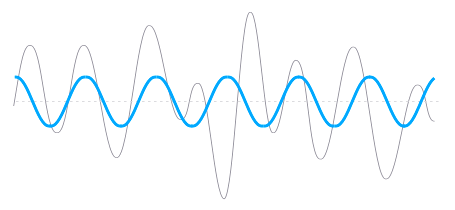
\includegraphics[scale=.88]{figuras/Interference1.png}
	}{
		\Fonte{Adaptado de \citeonline{yatebts2015}.}
	}
\end{figure}

\subsection{Desvanecimento (\textit{fading})}
\label{sub:desvanecimento}

O desvanecimento é um fenômeno causado pela variabilidade da intensidade do sinal no tempo associado à mobilidade da estação móvel \cite{haykin2008,rappaport2009}. Frequentemente, o sinal recebido é uma combinação de vários modos de propagação, resultantes da reflexão e da difração (detalhados anteriormente). Assim, a maior parte da comunicação acontece por espalhamento das ondas eletromagnéticas, que chegam de diferentes direções com diferentes atrasos de propagação \cite{haykin2008}. No receptor, o sinal final é a soma vetorial dessas ondas de caminhos múltiplos, podendo interagir umas com as outras construtiva ou destrutivamente, dependendo da amplitude e da fase de cada componente espectral \cite{haykin2008}.
\begin{figure}[H]
	\centering
	\Caption{\label{fig:fading}Interferência construtiva e destrutiva.}	
	\UECEfig{}{
		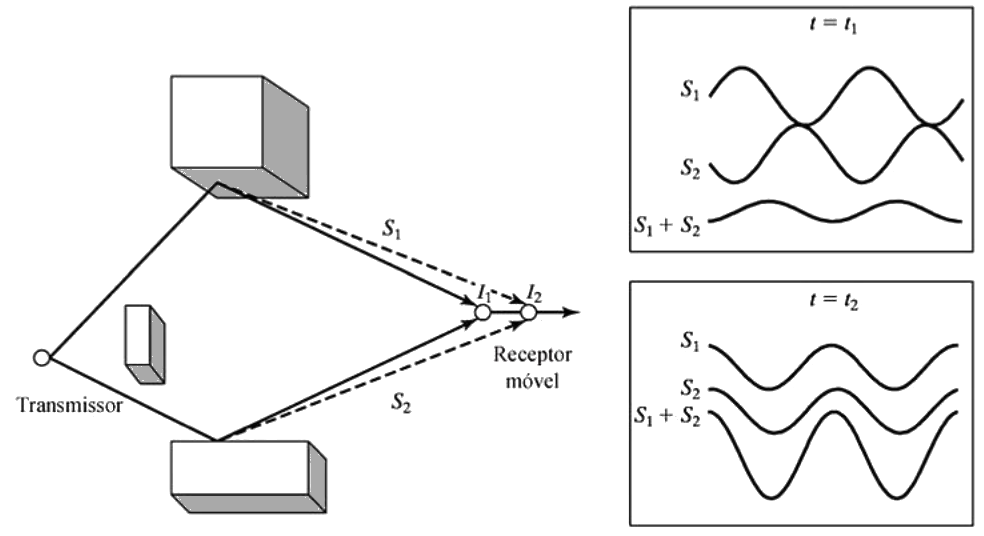
\includegraphics[scale=.4]{figuras/inter.png}
	}{
		\Fonte{\citeonline[p. ~57]{haykin2008}}
	}
\end{figure}

A rapidez com que as flutuações na magnitude do sinal ocorre pode ser classificada como desvanecimento lento ou desvanecimento rápido \cite{haykin2008}:

\begin{citacao}
	Desvanecimento lento surge do fato que a maioria dos grandes refletores e objetos difratores ao longo do percurso de transmissão estão distante do terminal. O movimento do terminal relativamente a esses objetos distantes é pequeno; consequentemente, as mudanças correspondentes na propagação são sentidas muito lentamente, Esses fatores contribuem para as perdas do percurso médio entre um transmissor fixo e um receptor fixo \cite{haykin2008}.
	
	Desvanecimento rápida surge da variação rápida dos níveis de sinal quando o terminal usuário move-se em distâncias curtas. O desvanecimento rápido é causado por reflexões de objetos e pelo movimento do terminal relativamente a esses objetos \cite{haykin2008}.
\end{citacao}

\section{Modelos de Propagação}
\label{sec:modelos-propagacao}

Para que se possa realizar um projeto de enlace de rádio confiável e com boa eficiência, são utilizados os chamados modelos de propagação. Os mesmos são desenvolvidos com base em medições empíricas que buscam alimentar com dados todo um processo matemático complexo capaz de representar a proliferação das ondas de rádio, predizer a perda de caminho ou a cobertura efetiva de um transmissor \cite{akpaida2018,najnudel2004}. Assim, é fácil concluir que, quanto mais informações for possível representar nestas equações, mais precisa será a caracterização do meio e seus efeitos \cite{akpaida2018}.

Modelos de propagação de rádio são empíricos por natureza. E como todos os modelos empíricos, os modelos de propagação de rádio não chamam a atenção para a conduta exata de uma conexão, mas sim para prever o comportamento que o \textit{link} pode mostrar sob as condições especificadas \cite{akpaida2018}.

Existem diversos modelos de propagação formulados por estudiosos e organizações voltadas para o ramo das comunicações sem fio. Cada modelo aplica-se a uma determinada situação específica, dependendo da característica física do local (região urbana ou região rural, por exemplo); frequência de operação do sistema de comunicação e o tipo de material da construção, fator esse, crítico para as redes Wi-Fi.

\subsection{Modelo de propagação no espaço livre}
\label{sub:espaco-livre}

O modelo de propagação no espaço livre é usado para prever a intensidade do sinal recebido quando o transmissor e o receptor possuem um linha de visão sem a presença de obstáculos, ou seja, quando há caminho livre entre eles \cite{rappaport2009}. Os sistemas de comunicação via satélite normalmente experimentam uma transmissão com caminho desobstruído.

O modelo de espaço livre, assim como a maioria dos modelos de propagação de radiofrequência, prevê que a potência recebida diminui em função da distância de separação transmissor-receptor (T-R) \cite{rappaport2009}. A potência no espaço livre recebida por uma antena receptora que está separada de uma antena transmissora, irradiando, por uma distância T-R é dada pela equação do espaço livre:
\begin{equation}
	\begin{aligned}
	\label{eq:friis}
		P_R = \dfrac{P_TG_TG_R}{L_P}
	\end{aligned}
\end{equation}

\noindent onde $P_T$ é a potência transmitida, $P_R$ E a potência recebida, $G_T$ é o ganho da antena transmissora, $G_R$ é o ganho da antena receptora e $L_P$ é a perda do percurso entre T-R. Tanto a dedução matemática do ganho ($G$) da antena quanto a da \emph{perda do percurso} ($L_P$) pode ser encontrada com detalhes em \citeonline{haykin2008}.

A equação \ref{eq:friis} é conhecida como \emph{equação de Friis}. É possível simplificá-la em função do ganho em decibel (dB) \cite{haykin2008}:
\begin{equation}
	\begin{aligned}
	\label{eq:friis-decibel}
		P_R(dB) = P_T(dB) + G_T(dB) + G_R(dB) - L_P(dB)
	\end{aligned}
\end{equation}

\noindent onde $X(dB) = 10\log_{10} (X)$. A \emph{equação de Friis} é a equação fundamental para o planejamento do enlace de rádio, pois relaciona as potências transmitida e recebida, considerando as condições da transmissão \cite{haykin2008}. Ela fornece os requisitos essenciais para que o nível de potência requerida pelo receptor seja suficiente para ele detectar as informações transmitidas com confiabilidade \cite{haykin2008}.

\subsection{Modelo de dois raios}
\label{sub:modelo-2-raios}

A equação do espaço livre (Equação \ref{eq:friis}) considera que sempre existe uma linha de visada direta entre transmissor e receptor, não considera, entretanto, o efeito da superfície terrestre na comunicação. Esse fato raramente acontece com transmissões em solo, o que torna, o modelo de espaço livre impreciso na grande maioria dos casos \cite{rappaport2009}.

O modelo de reflexão no solo (Figura \ref{fig:2raios}), baseado na ótica geométrica, considera o caminho direto e um caminho de propagação refletido no solo entre o transmissor e o receptor \cite{rappaport2009}.
\begin{figure}[H]
	\centering
	\Caption{\label{fig:2raios}Modelo de reflexão no solo com dois raios.}	
	\UECEfig{}{
		\fbox{\begin{varwidth}{\dimexpr\textwidth-2\fboxsep-2\fboxrule\relax}
		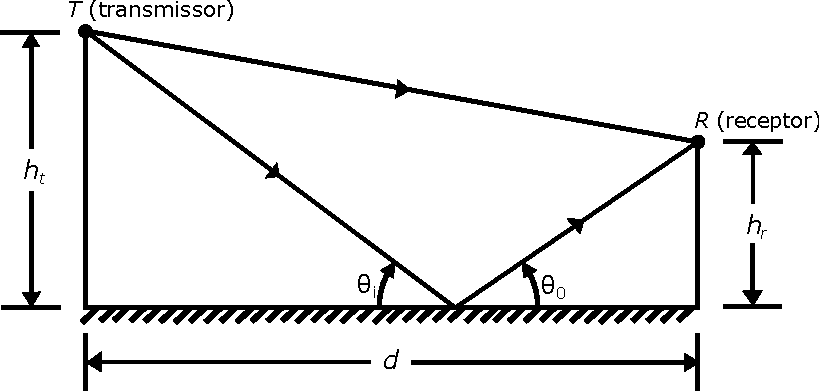
\includegraphics[scale=.8]{figuras/modelo2raios.pdf}
		\end{varwidth}}
	}{
		\Fonte{Adaptado de \citeonline[p. ~80]{rappaport2009}}
	}
\end{figure}

A potência recebida a uma distância $d$ do transmissor para o modelo de dois raios pode ser expressa como \cite{rappaport2009}:
\begin{equation}
	\begin{aligned}
	\label{eq:2-raios}
		P_R = P_TG_TG_R\dfrac{h^2_Th^2_R}{d^4}
	\end{aligned}
\end{equation}

\noindent onde $P_R$ é a potência recebida, $P_T$ é a potência transmitida, $G_T$ é o ganho da antena transmissora, $G_R$ é o ganho da antena receptora, $h_T$ é a altura do transmissor e $h_R$ é a altura do receptor. Todo o desenvolvimento algébrico até chegar a Equação \ref{eq:2-raios} pode ser encontrada em \citeonline{rappaport2009} ou \citeonline{haykin2008}.

\subsection{Modelo log-distância (log simplificado)}
\label{sub:log-distancia}

Os modelos de propagação baseados em medições em campo indicam que que a potência média do sinal recebida cai logaritmicamente com a distância, seja em enlaces de rádio para ambientes \textit{indoor} ou \textit{outdoor} \cite{rappaport2009}. A perda de percurso média para a uma separação T-R qualquer é obtida em função da distância usando um expoente de perda de caminho, $n$, dada por
\begin{equation}
	\begin{aligned}
	\label{eq:log-distancia}
		PL(d) \propto \left(\dfrac{d}{d_0}\right)^n
	\end{aligned}
\end{equation}

\noindent ou

\begin{equation}
	\begin{aligned}
	\label{eq:log-distancia-2}
		PL(dB) = PL(d_0) + 10n\log_{10}\left(\dfrac{d}{d_0}\right)^n
	\end{aligned}
\end{equation}

\noindent onde $PL$ é a perda média do percurso, $n$ é o expoente de perda de caminho (indica a velocidade com a qual essa perda aumenta com relação a distância), $d_0$ é a distância de referência próxima que é determinada pelas medições perto do transmissor, e $d$ é a distância de separação T-R.

\subsection{Modelo de Okumura--Hata}
\label{sub:okumura-hata}

A melhor aplicação do modelo de Okumura-Hata acontece na faixa de frequência existente entre 150 MHz e 1 GHz, podendo ser estendido até 1,5 GHz \cite{haykin2008,rappaport2009}. Os dados originais foram medidos por Okumura (entre outros) em diversos locais do Japão. Algum tempo depois, Hata forneceu a equação para predição da perda de propagação em área urbana, juntamente com outras equações de correção para aplicações em área suburbana e aberta.

As perdas do percurso, em dB, para esses três tipos de meios, respectivamente, são dadas pelas equações
\begin{equation}
\begin{split}
	\label{eq:okumura-hata}
		L_P & = A + B\log_{10}r \\
		L_P & = A + B\log_{10}r - C \\
		L_P & = A + B\log_{10}r - D
\end{split}
\end{equation}

\noindent onde $r$ é o alcance em quilômetros, os parâmetros $A$, $B$, $C$ e $D$ dependem da frequência de operação ($f_c$), da altura da estação transmissora ($h_b$) e da altura da estação receptora ($h_m$). As fórmulas que permitem-nos determinar os valores de $A$, $B$, $C$ e $D$ encontram-se na literatura \cite{haykin2008}.

\subsection{Modelo Multi--Wall--and--Floor}
\label{sub:modelo-MWF}

O modelo \emph{Multi-Wall-and-Floor} (MWF) leva em consideração a perda decrescente de penetração de paredes/pisos da mesma categoria, à medida que o número de paredes/pisos atravessados aumenta, isto é, defende que a relação entre as  perdas não segue uma linearidade lógica \cite{lott2001ieee}. Por exemplo, dada uma perda de penetração de 2 dB em uma parede de concreto, essa mesma onda, ao penetrar em outra parede de mesma característica, não sofrerá uma atenuação de 2 dB como ocorrido no primeiro obstáculo.

O modelo MWF, proposto por \citeonline{lott2001ieee}, é voltado especialmente para a análise dos efeitos da propagação em ambientes fechados (\textit{indoor}), pois esses locais concentram grande variedade de divisórias construídas com diferentes materiais. A perda sofrida por uma onda de rádio ao propagar-se por múltiplas paredes/pisos, $L_{MWF}$, pode ser dada pela seguinte equação:
\begin{equation}
	\begin{aligned}
	\label{eq:mwf}
		L_{MWF} = L_0 + 10n\log_{10}(d) + \sum_{i=1}^{I} \sum_{k=1}^{K_{wi}} L_{wik} + \sum_{j=1}^{J} \sum_{k=1}^{K_{fj}} L_{fjk}
	\end{aligned}
\end{equation}

\noindent onde $L_0$ é a perda de trajetória a uma distância de 1 m, $n$ é o fator de perda do percurso, $d$ é a distância entre o transmissor e o receptor, $L_{wik}$ é a atenuação devido ao tipo de parede $i$ e à $k$-ésima parede atravessada, $L_{fjk}$ é a atenuação devida ao tipo de piso $j$ e ao $k$-ésimo piso atravessado, $I$ é o número de tipos de parede, $J$ é o número de tipos de piso, $K_{wi}$ é o número de paredes atravessadas do tipo $i$ e $K_{fj}$ é o número de paredes atravessadas do tipo $j$.

	
	% Elementos pós-textuais
	
	% IMPORTANTE!!!
	%% SEGUIR A SEGUINTE ORDEM DE EXECUÇÃO DOS ARQUIVOS PARA AS REFERÊNCIAS: 
	% 1 - COMPILAR ARQUIVO .TEX (1X)
	% 2 - COMPILAR ARQUIVO .BIB (1X)
	% 3 - COMPILAR ARQUIVO .TEX (2X)
%	Marc, eu parei de usar o abntex2, mas se bem me lembro é o \nocite{*}
%que não funciona, \nocite{referencia-especifica} funciona. Você pode
%acrescentar ao seu documento um comando \nocite para cada referência
%desejada.
	% Caso utilze o TeXstudio não é necessário seguir as etapas anteriores.
	\bibliography{elementos-pos-textuais/referencias}
	
	
%	\imprimirglossario	
%	\imprimirapendices
%		% Adicione aqui os apendices do seu trabalho
%		\apendice{Lorem Ipsum}
\label{ap:lorem-ipsum}

\lipsum[1]
%		\apendice{Modelo de Capa}
\label{ap:modelo-de-capa}

\lipsum[1]

%		\apendice{Termo de Fiel Depositário}
\label{ap:termo-de-fiel-depositario}

\noindent \textbf{Pesquisa:} ANÁLISE DA MORTALIDADE INFANTIL COM MALFORMAÇÕES CONGÊNITAS.

\noindent Pelo presente instrumento que atende às exigências legais, a Sra. Maria Consuelo Martins Saraiva, ``fiel depositário'' com o cargo de Secretária Municipal de Saúde de Iracema, após ter tomado conhecimento do protocolo de pesquisa intitulado: ANÁLISE DA MORTALIDADE INFANTIL COM MALFORMAÇÕES CONGÊNITAS. Analisando a repercussão desse estudo no contexto da saúde pública e epidemiologia, autoriza Karla Maria da Silva Lima, enfermeira, aluna do Curso de Mestrado Acadêmico em Enfermagem da Universidade Estadual do Ceará (UECE), sob orientação do Prof. Dr. José Maria de Castro, da UECE, ter acesso aos bancos de dados do Sistema de Informação sobre Nascidos Vivos e do Sistema de Informação sobre Mortalidade da Secretaria Municipal de Saúde de Iracema, objeto deste estudo, e que se encontram sob sua total responsabilidade. Fica claro que o Fiel Depositário pode a qualquer momento retirar sua AUTORIZAÇÃO e ciente de que todas as informações prestadas tornar-se-ão confidenciais e guardadas por força de sigilo profissional, assegurando que os dados obtidos da pesquisa serão somente utilizados para estudo.	
%	\imprimiranexos
%		% Adicione aqui os anexos do seu trabalho
%		\anexo{Exemplo de Anexo}
\label{an:exemplo-de-anexo}

\lipsum[13]		
%		\anexo{Dinâmica das classes sociais}
\label{an:dinamica-das-classes-sociais}

\lipsum[14]
\index{AAA}
%	\imprimirindice
\end{document}